\chapter{Running Examples}
\section{Public functions of PNIS}
This section presents parts of the implemented GUI of the PNIS system exposing publicly available functions. 
\subsection{Landing Page}
The landing page serves as the main entry point to the application (see figure~\ref{fig:landingPage}). It provides guests with a simple interface to begin their exploration. Guests can search for places using the search bar.
\begin{figure}[htb]
    \centering
    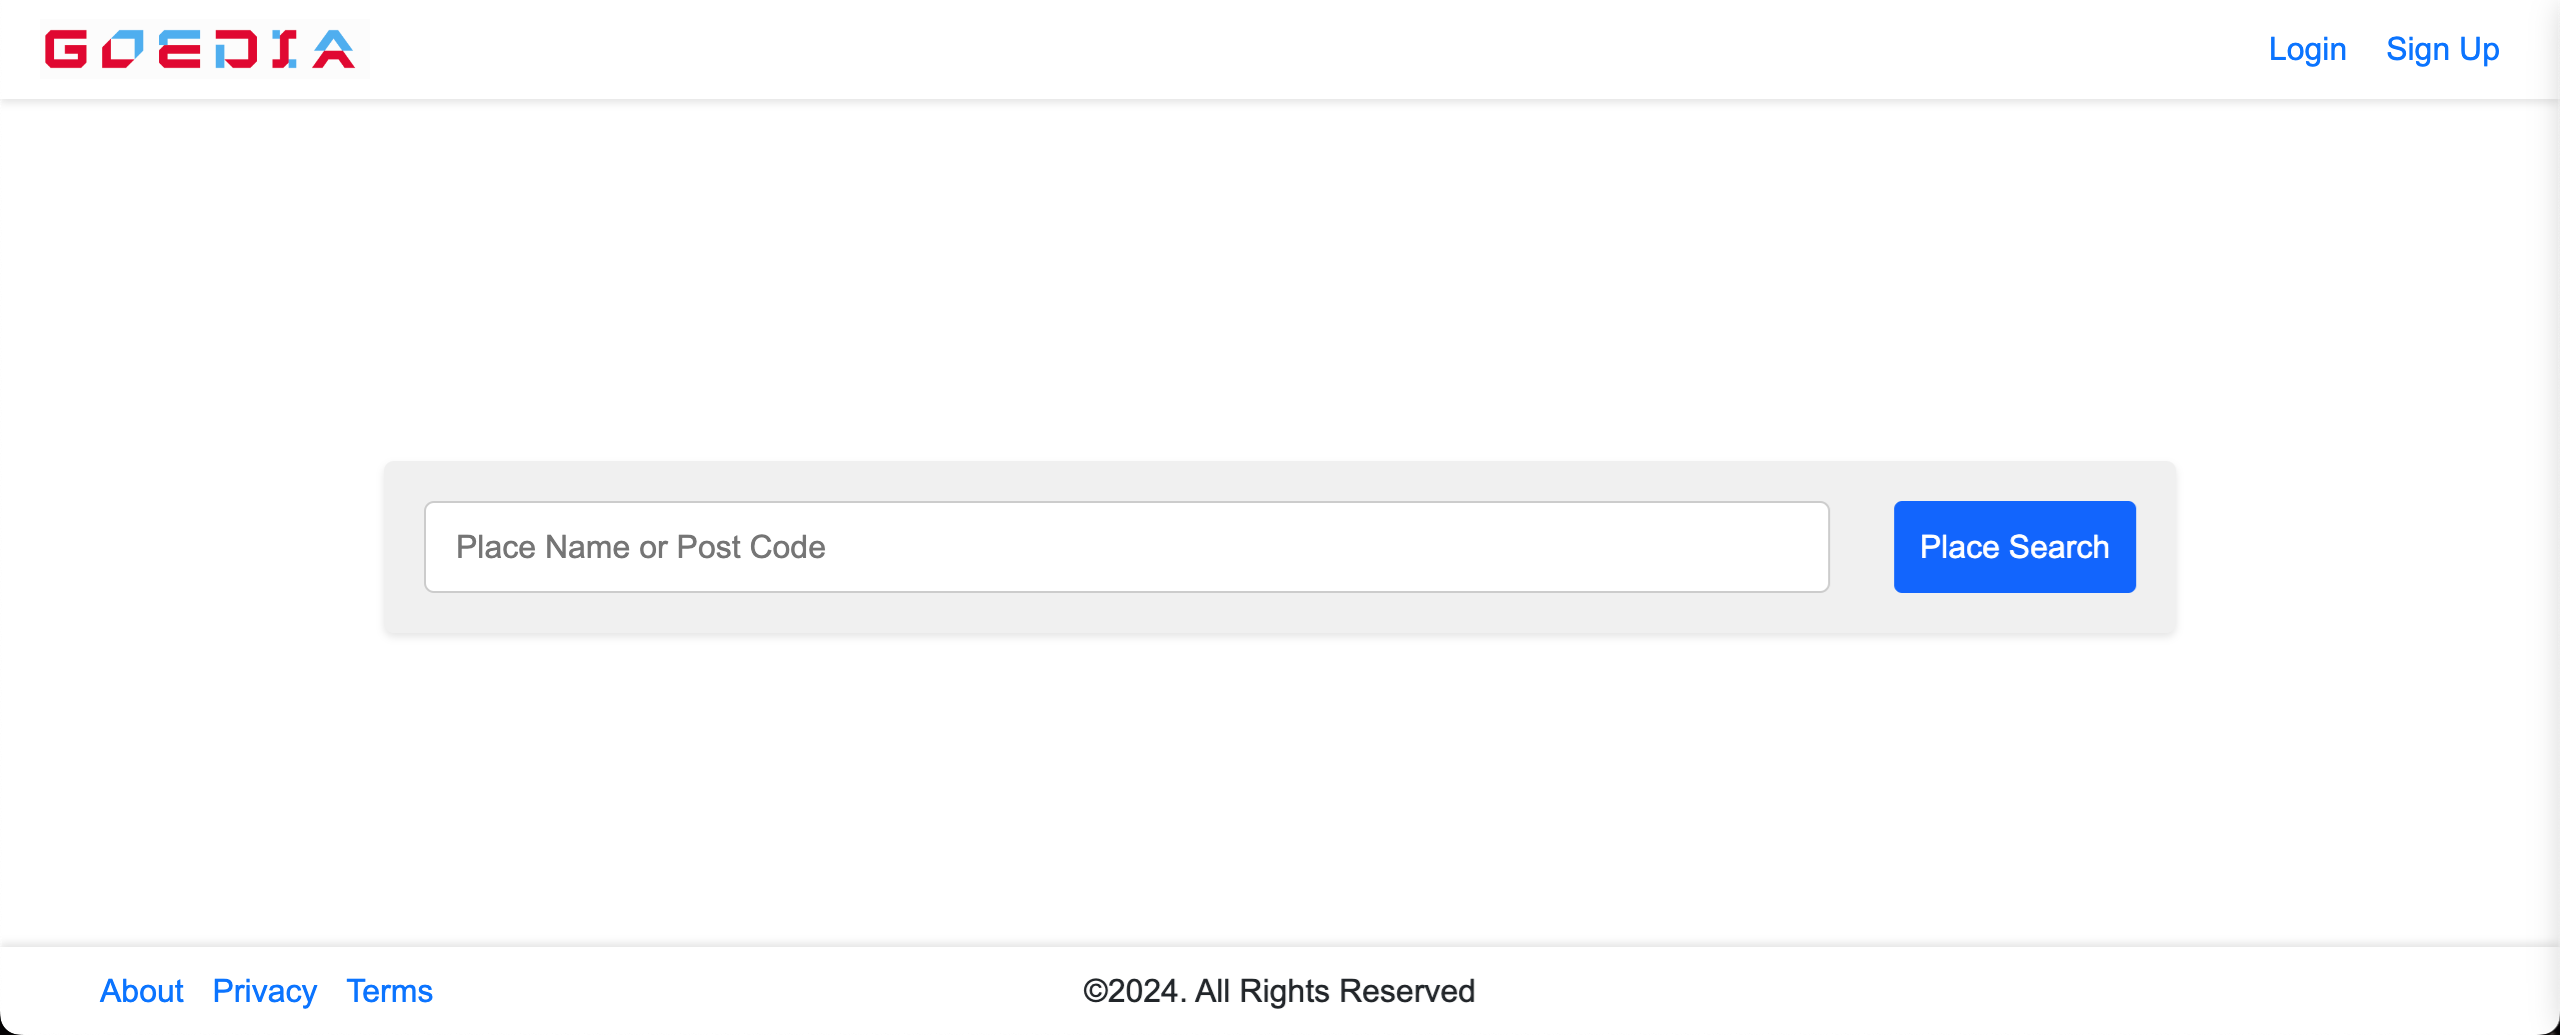
\includegraphics[width=\textwidth]{landingPage.png}
    \caption{Landing Page}
    \label{fig:landingPage}
\end{figure}

Guests can search for places without needing to log in. The search bar allows them to type in the name of a place, and suggestions are provided as they type (see figure~\ref{fig:guestSearch}).
\begin{figure}[htb]
    \centering
    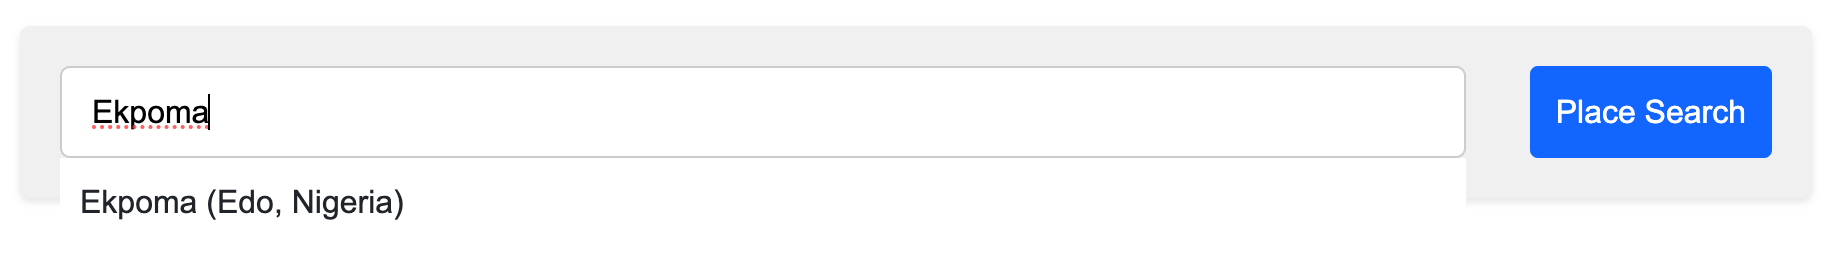
\includegraphics[width=.6\textwidth]{guestSearch.png}
    \caption{Guest Search}
    \label{fig:guestSearch}
\end{figure}

\subsection{Place Details}
When a place is selected, detailed information about it is displayed, including a map that allows for interactive use to see where exactly the place is located, and also other information such as the year it was founded, population, elevation, pronunciation of the name and a description with a button to see more details (see figure~\ref{fig:placeDetails}).

\begin{figure}[htb]
    \centering
    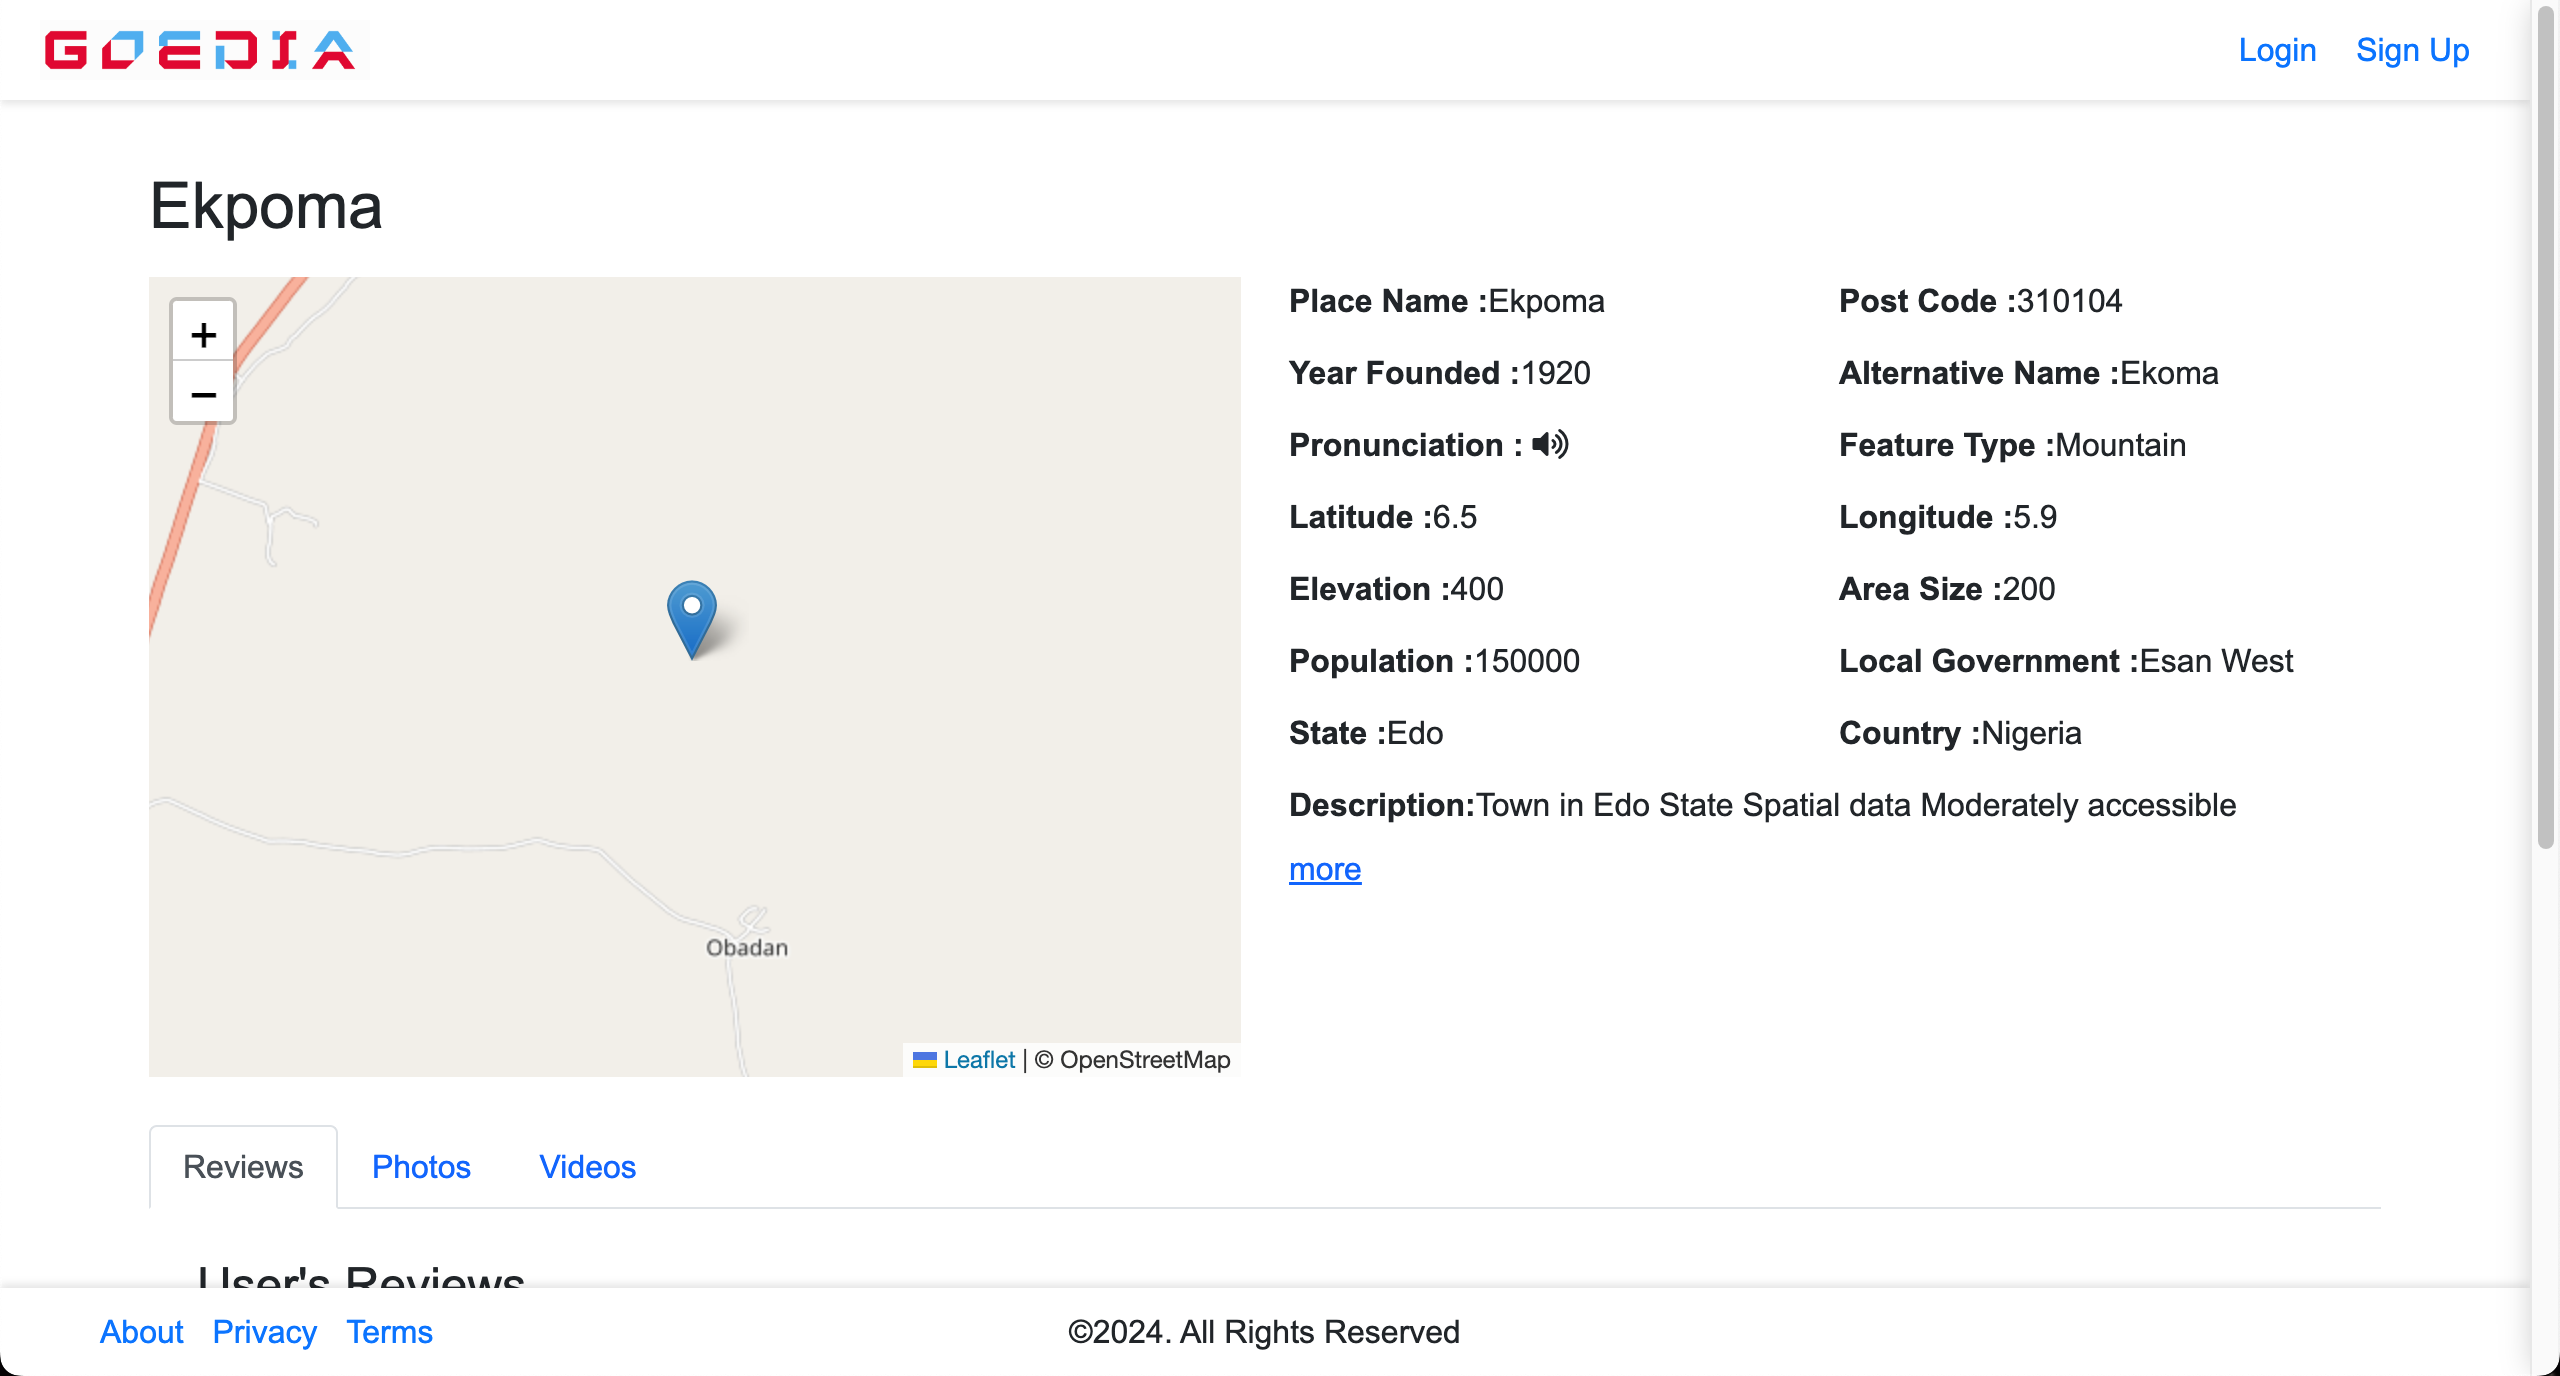
\includegraphics[width=\textwidth]{placeDetails.png}
    \caption{Place Details}
    \label{fig:placeDetails}
\end{figure}

\subsection{More Details}
Guests can delve into additional details about a place, including alternative names of the place with a voice recording (see figure~\ref{fig:moreDetails}).

\begin{figure}[htb]
    \centering
    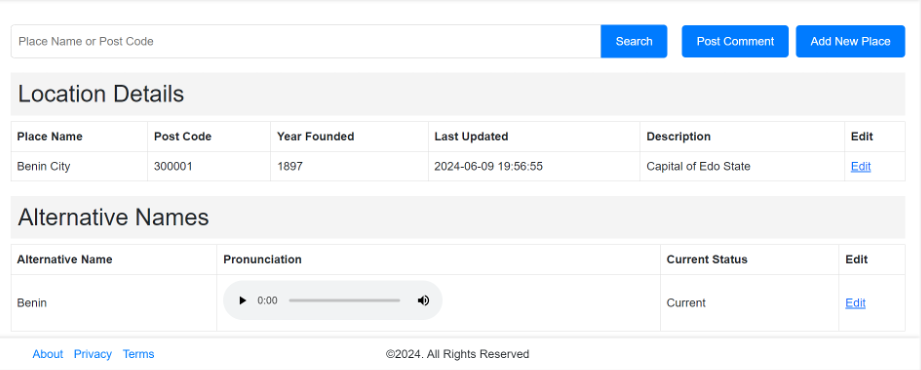
\includegraphics[width=\textwidth]{moreDetails.png}
    \caption{More Details}
    \label{fig:moreDetails}
\end{figure}

\subsection{Geographical Features}
This section provides geographical data about the place, such as its feature type, location, elevation, area size, and population. This information is useful for understanding the physical characteristics of the place (see figure~\ref{fig:moreDetails2Geo}). Additionally, declared administrative details with periodic data is available in the tables.

\begin{figure}[htb]
    \centering
    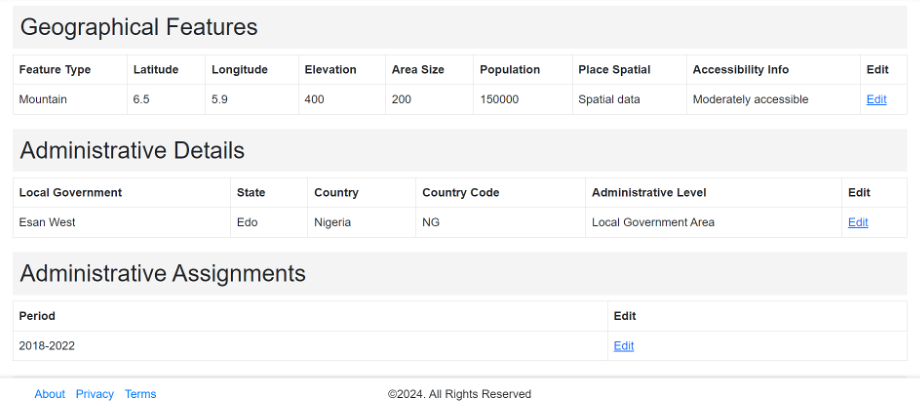
\includegraphics[width=\textwidth]{moreDetails2Geo.png}
    \caption{Geographical Features}
    \label{fig:moreDetails2Geo}
\end{figure}

\section{Historical Data}
Significant events that shaped place identity can be seen under the historical data table (see figure~\ref{fig:moreDetails3AdmDetails}). This may help a better understanding of the place by giving a historical context.

\begin{figure}[htb]
    \centering
    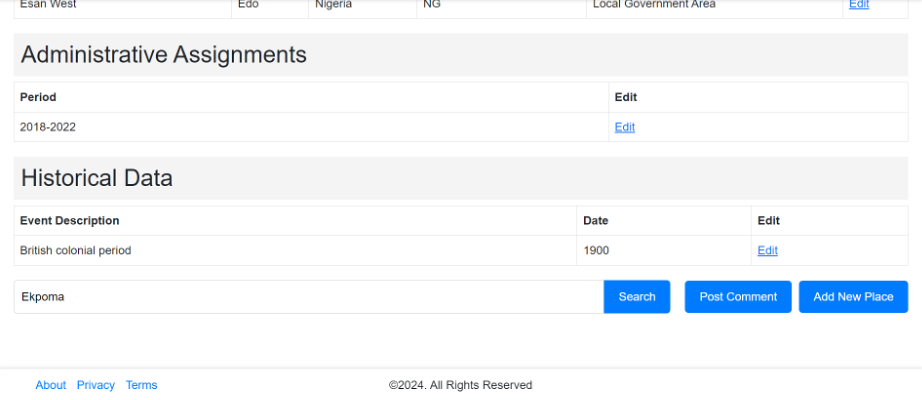
\includegraphics[width=\textwidth]{moreDetails3AdmDetails.png}
    \caption{Administrative Details}
    \label{fig:moreDetails3AdmDetails}
\end{figure}

\section{Protected functions of PNIS}
This section presents parts of the implemented GUI of the PNIS system with protected functions. 

\subsection{User access}
New users can sign up by providing their full name, email address, password, and date of birth (see figure~\ref{fig:useraccess}a). After that they can start contributing to the platform.

When guests click on either post comment or add new place buttons on place details page or use the navigation buttons on the header they are redirected to the authorization page. If they already have an account, they can log in using their email address and password (see figure~\ref{fig:useracces}b). 
\begin{figure}[htb]
    \centering
		\begin{tabular}{ll}
		a) & b) \\
    \vtop{\vskip-2ex\hbox{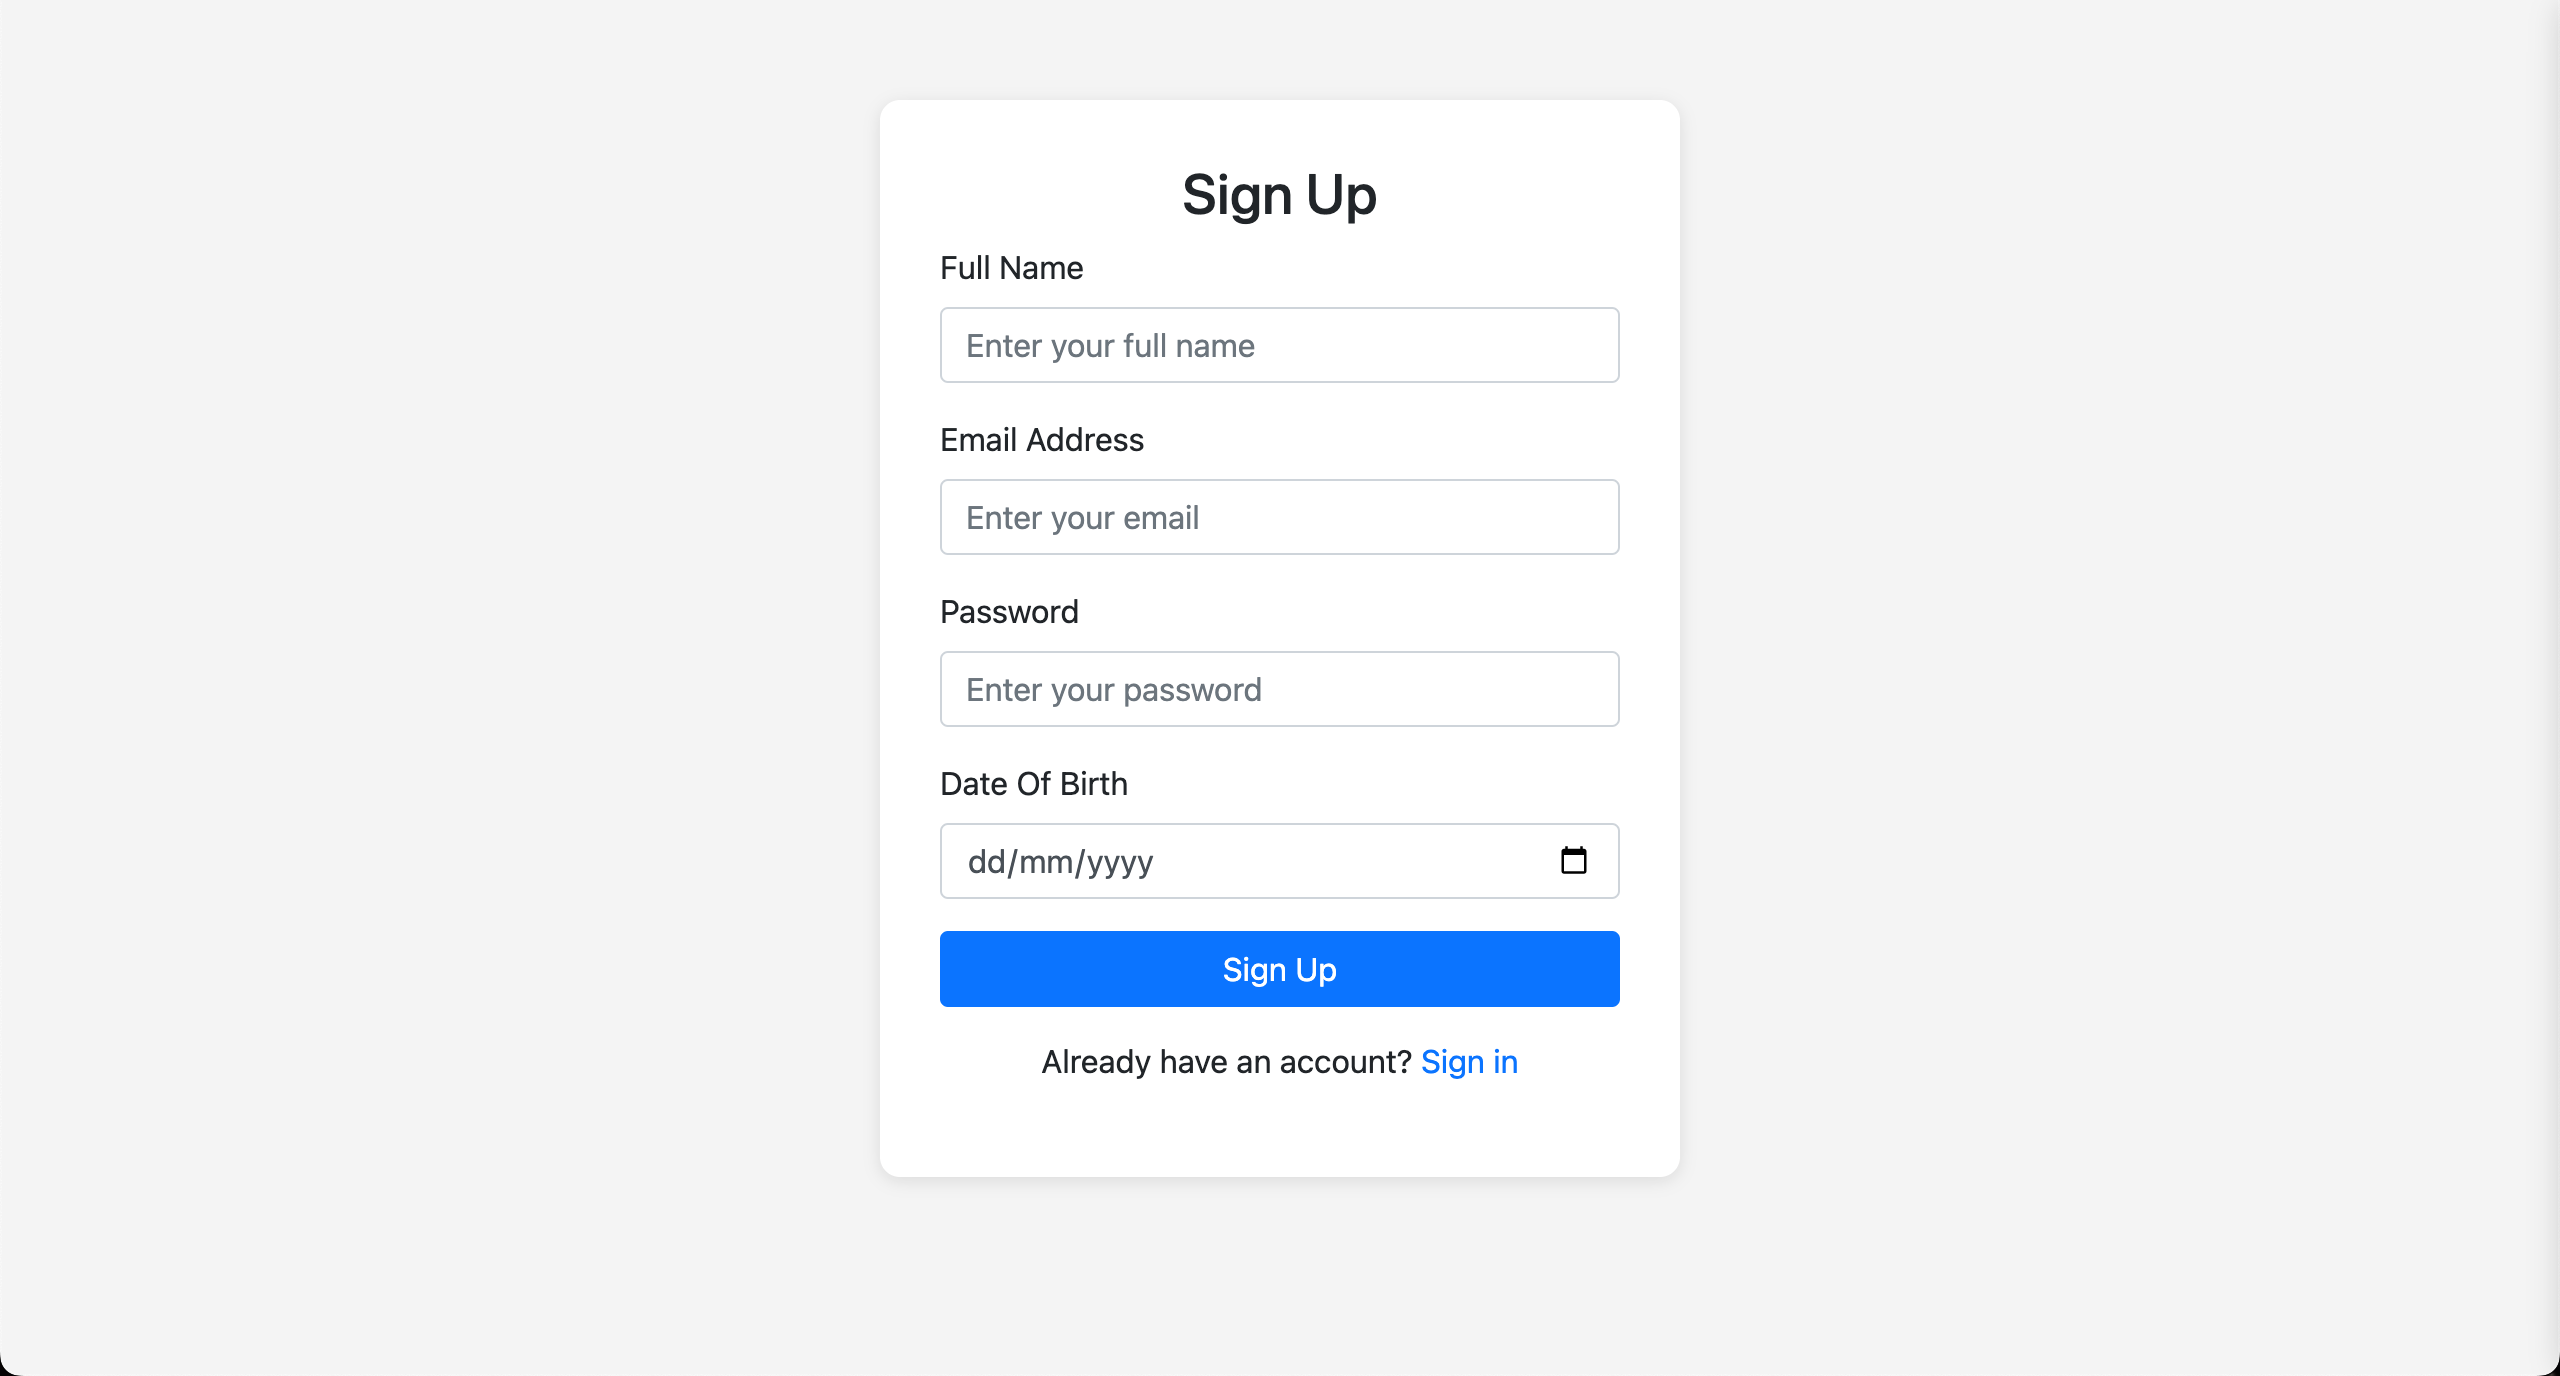
\includegraphics[width=0.4\textwidth]{signup.png}}}
		& 
		\vtop{\vskip-2ex\hbox{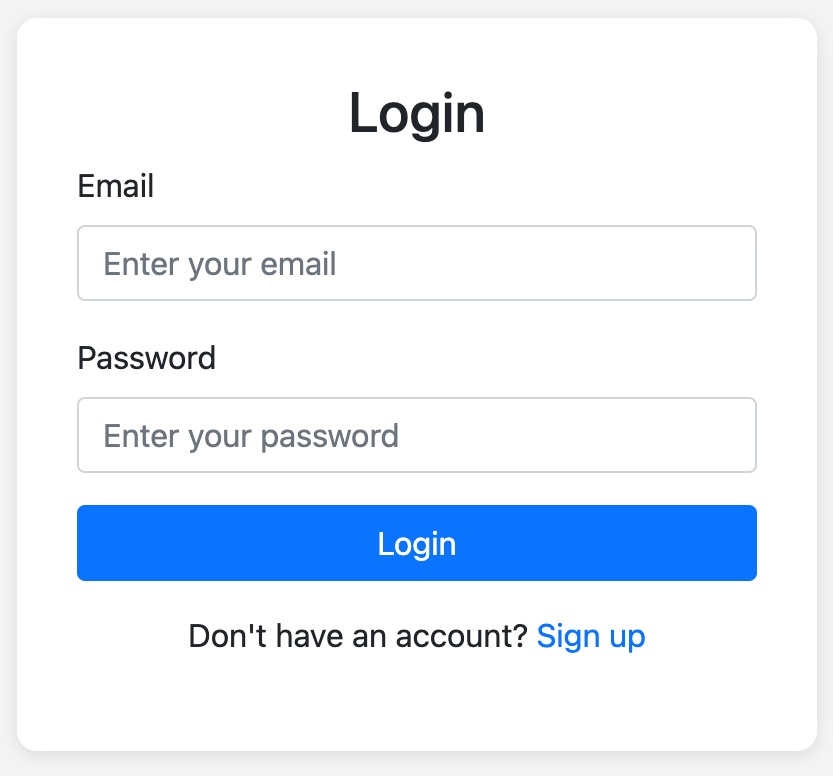
\includegraphics[width=0.4\textwidth]{login.png}}}
		\end{tabular}
    \caption{User access: a) registration; b) login}
    \label{fig:useraccess}
\end{figure}


\subsection{Contributing data}
Users can add new places by filling in basic information such as the place name, post code, year founded, and a brief description (see figure~\ref{fig:addnewPlace}a).

Users should also provide alternative names for a place, along with their pronunciation with a voice recording (see figure~\ref{fig:addnewPlace}b). This section also includes options to indicate if the name is currently in use and to add historical data.
\begin{figure}[htb]
    \centering
		\begin{tabular}{ll}
		a) & b) \\
    \vtop{\vskip-2ex\hbox{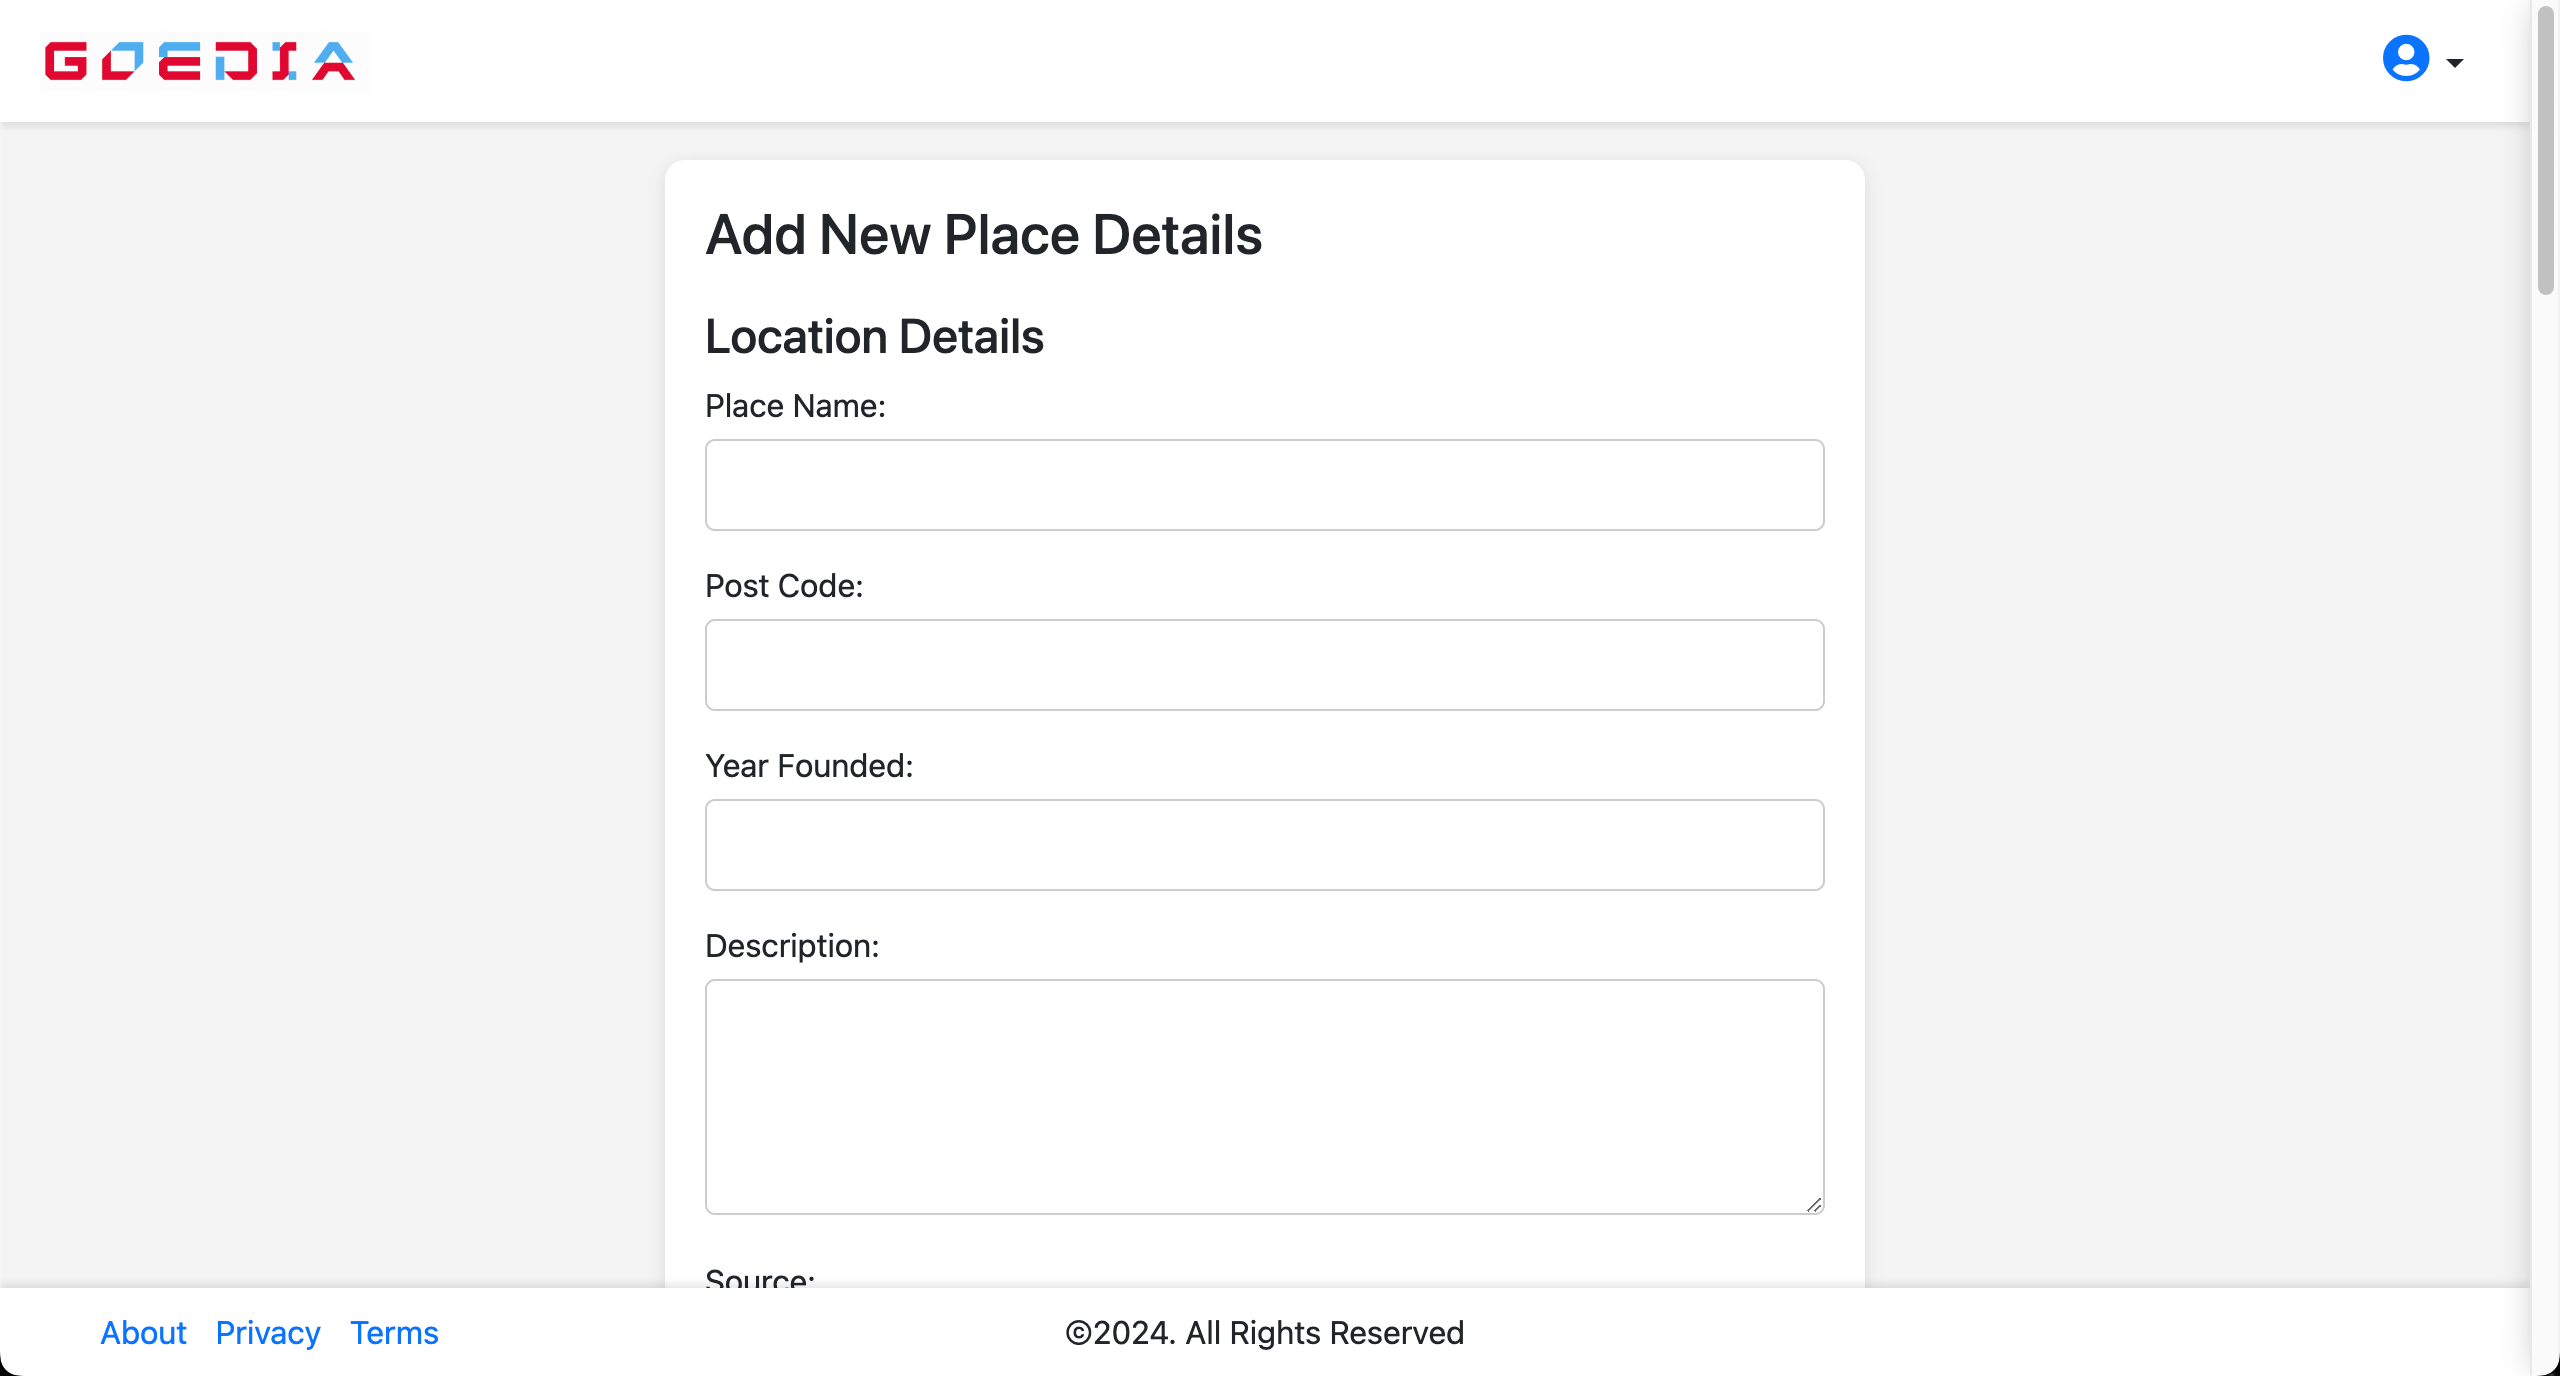
\includegraphics[width=0.4\textwidth]{addnewPlace.png}}}
		& 
		\vtop{\vskip-2ex\hbox{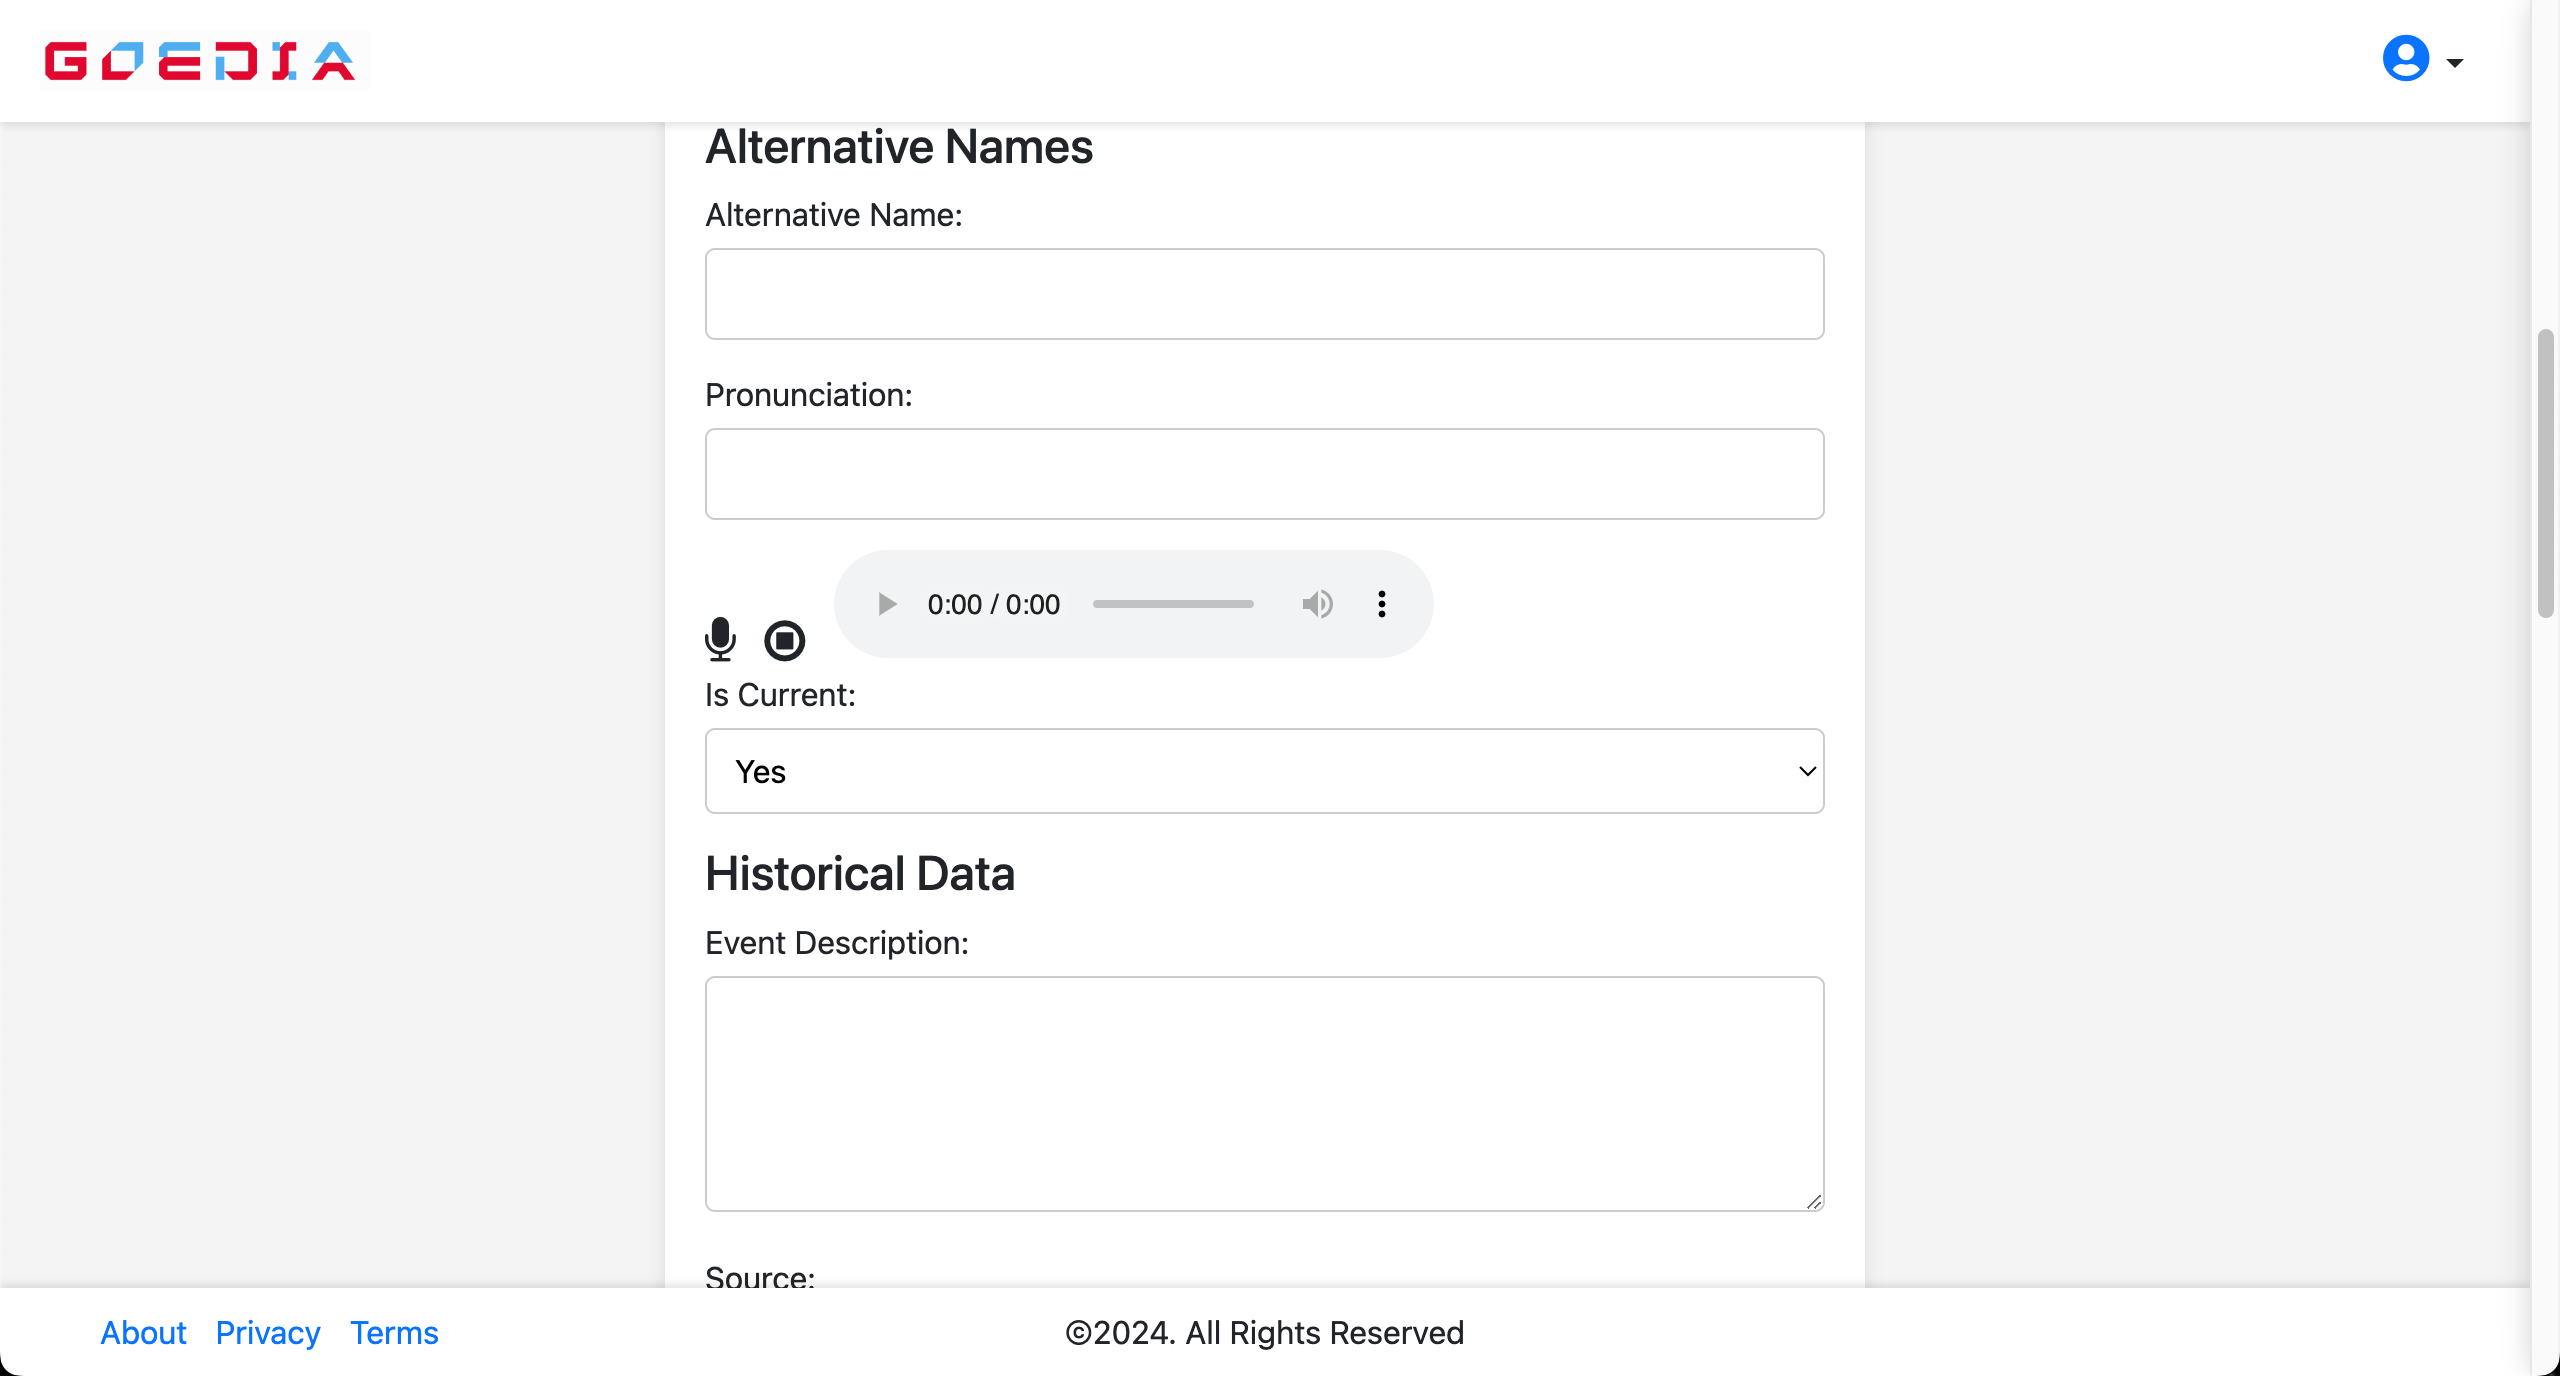
\includegraphics[width=0.4\textwidth]{addnewPlaceAlternativeName.png}}}\\
	  c) & d) \\
    \vtop{\vskip-2ex\hbox{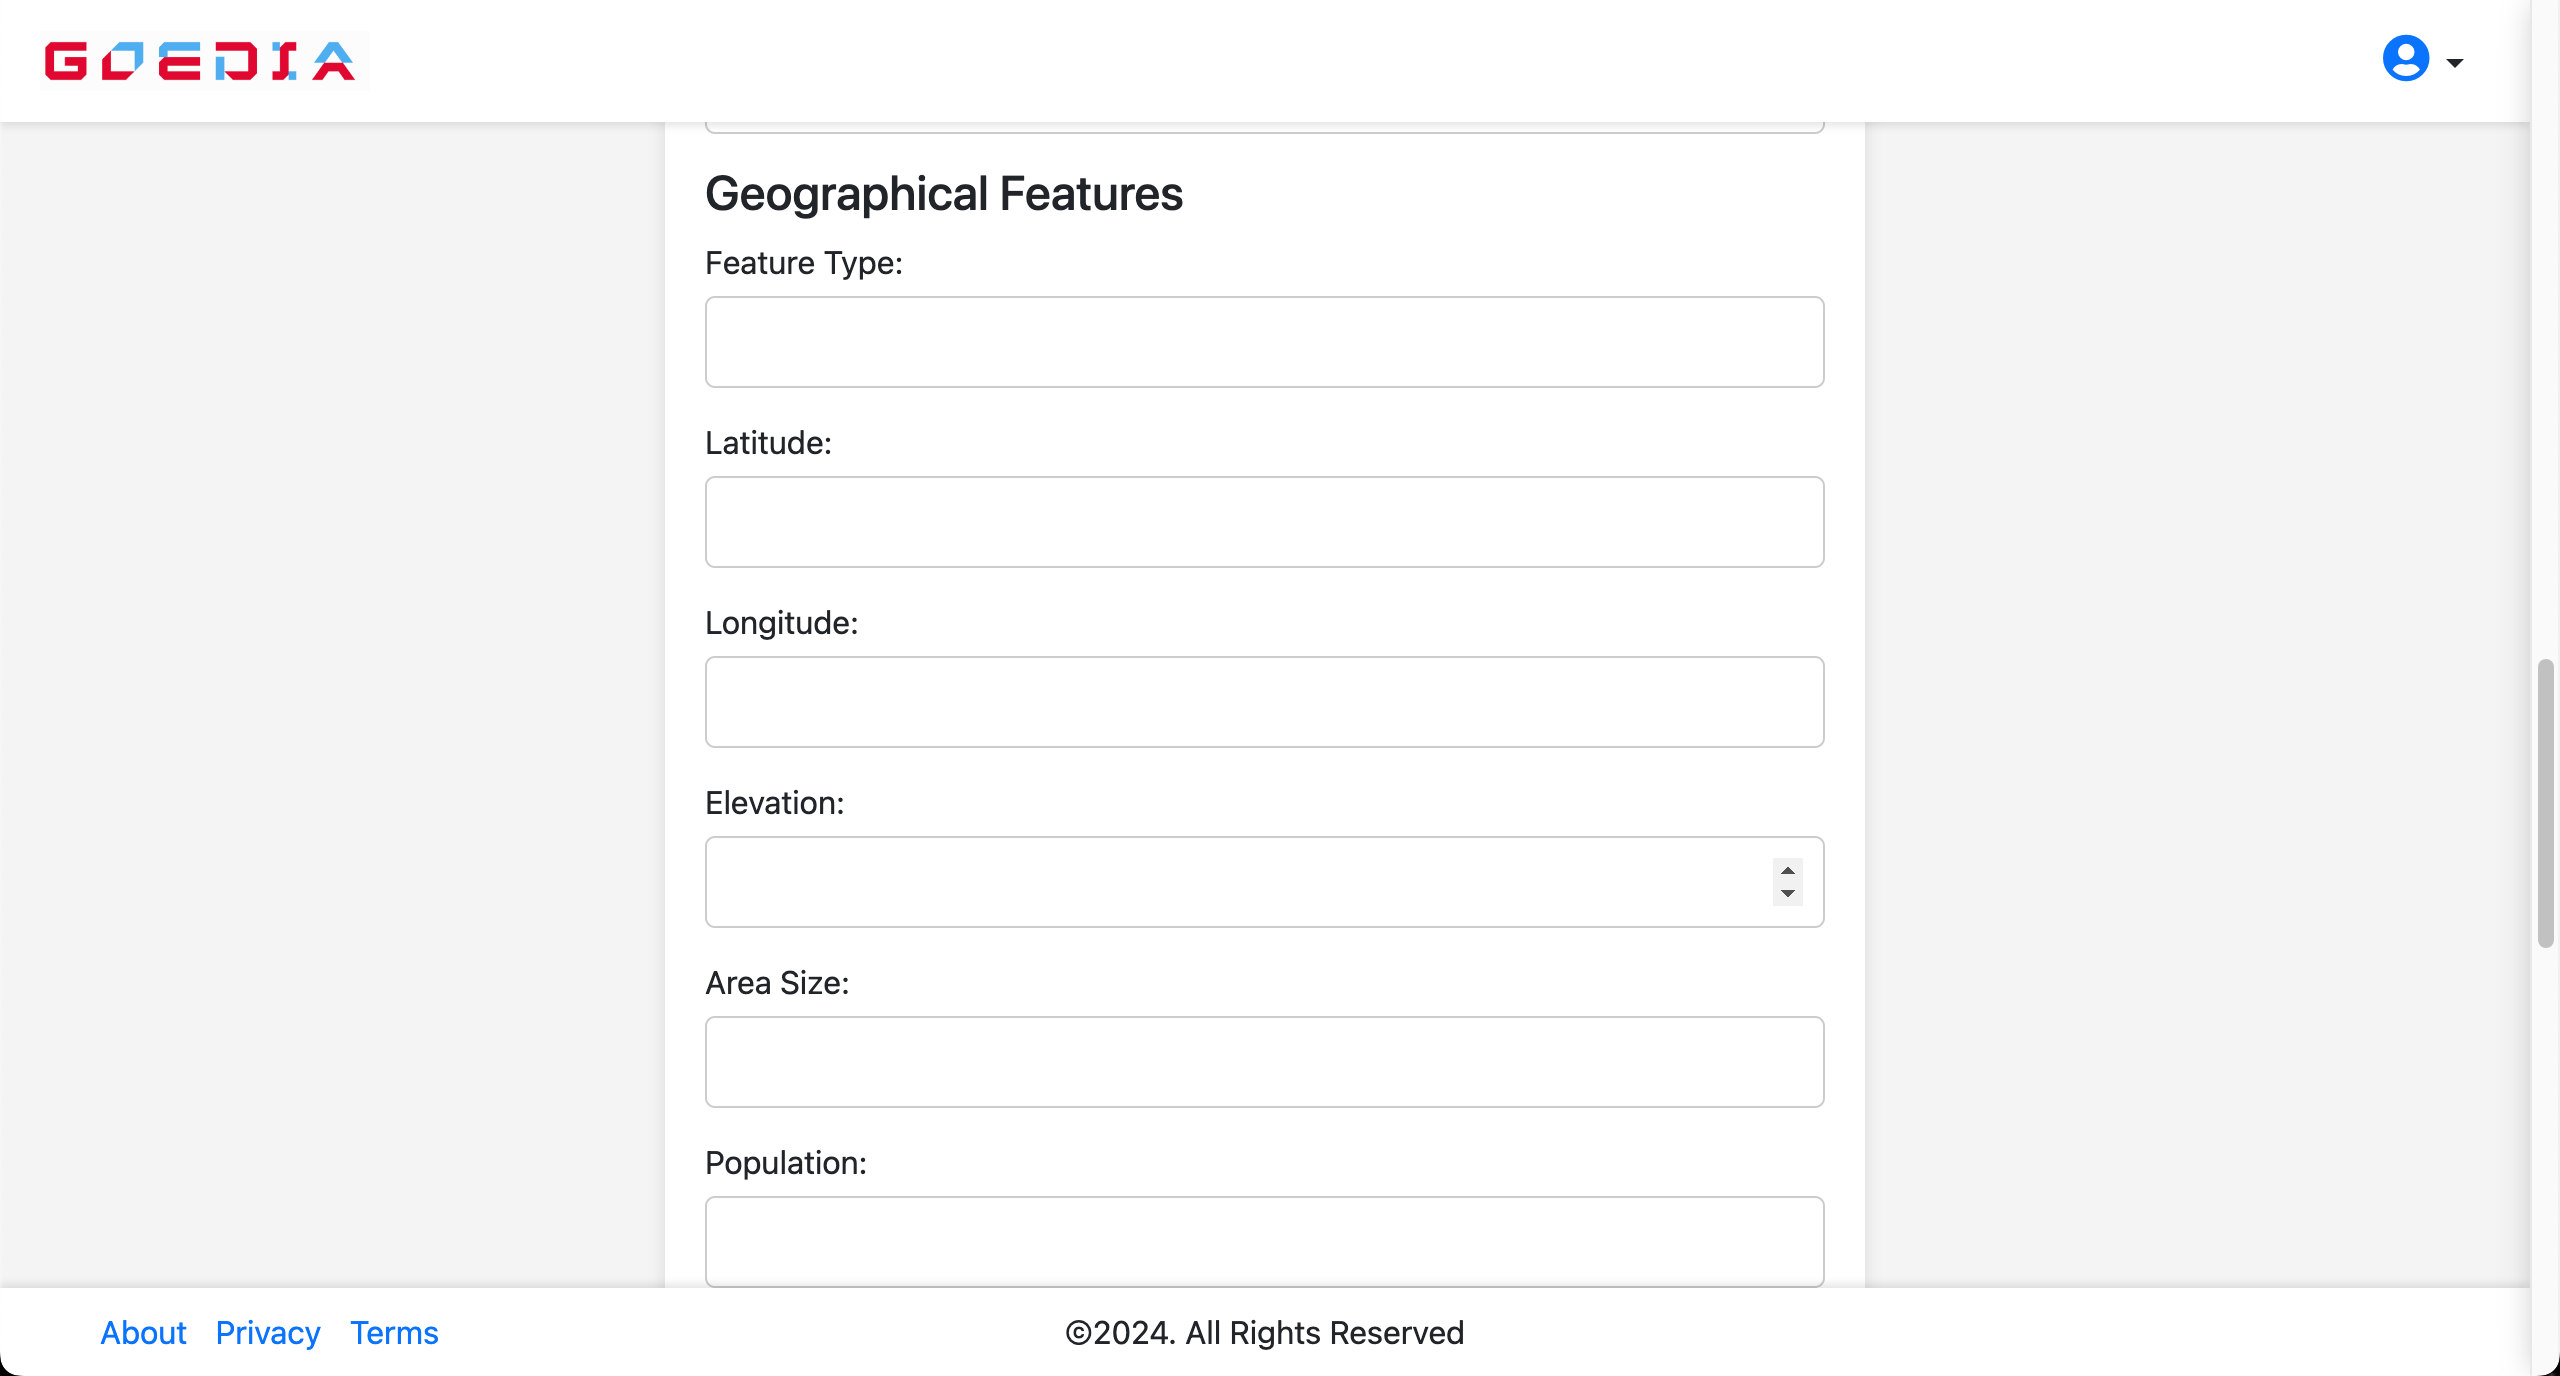
\includegraphics[width=0.4\textwidth]{addnewPlaceGeo.png}}}
		& 
		\vtop{\vskip-2ex\hbox{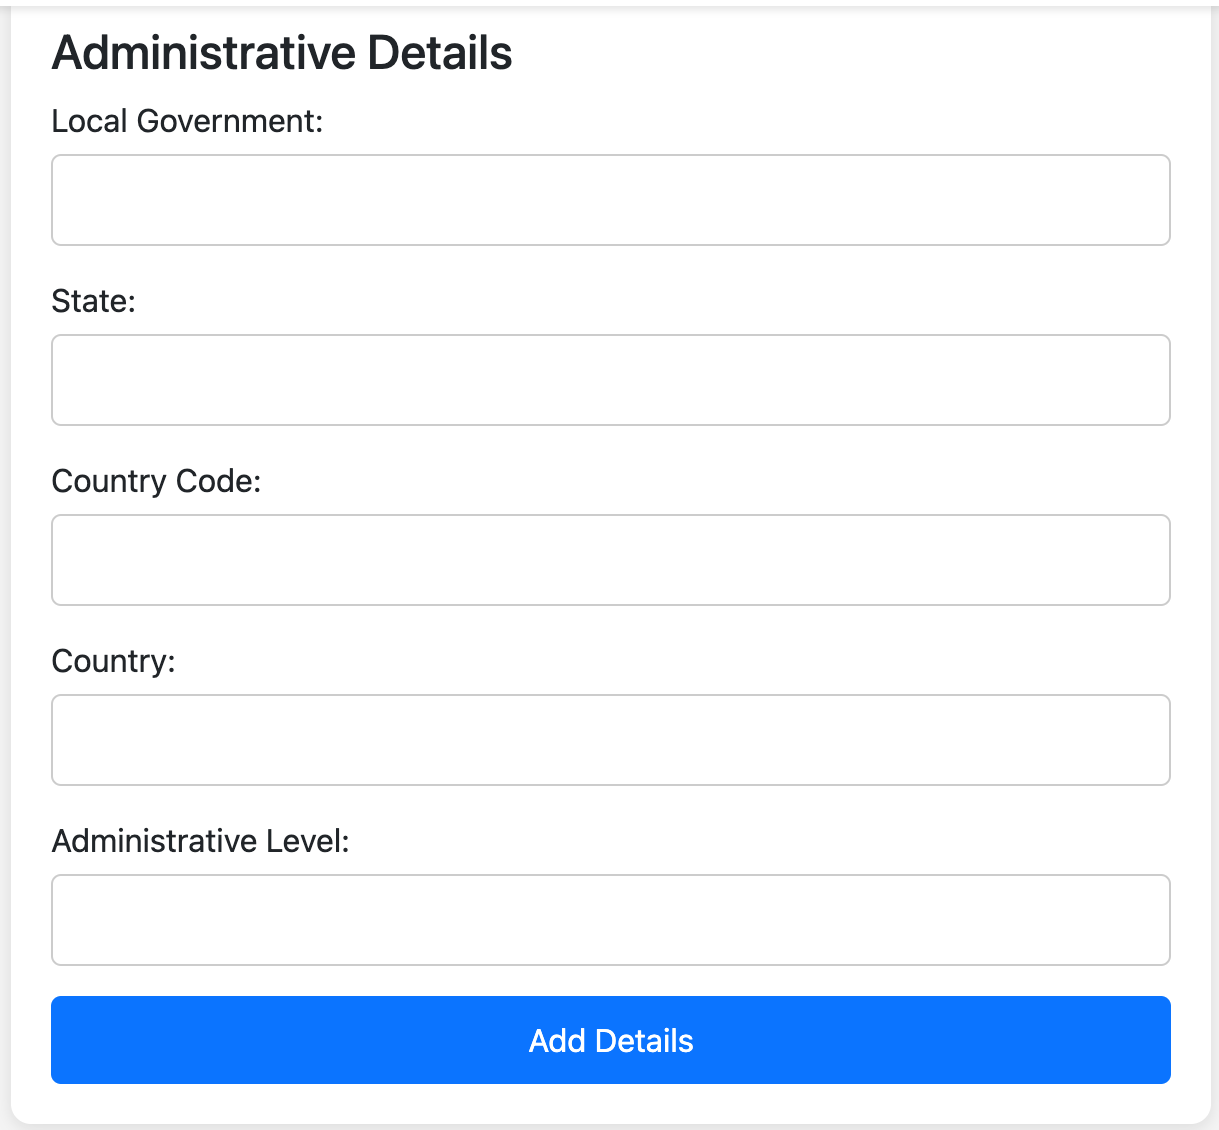
\includegraphics[width=0.4\textwidth]{addNewPlaceAdmDetails.png}}}
		\end{tabular}
    \caption{Contributing data: a) basic information; b) alternative names; c) geographical features; d)~administrative details}
    \label{fig:addnewPlace}
\end{figure}

Geographical details such as the feature type, latitude, longitude, elevation, area size, and population are entered here to give a comprehensive understanding of the place's physical characteristics (see figure~\ref{fig:addnewPlace}c).

Users can add administrative details such as the local government, state, country code, country, and administrative level to provide more context about the governance of the place (see figure~\ref{fig:addnewPlace}d).

\subsection{Experience Feed}
Users can view and share their experiences about different places to help others learn more about them.
The feed displays user posts along with the date and time they were shared, providing a platform for users to share their stories and insights together with photos and videos (see figure~\ref{fig:experienceFeed}a).

Users can post their personal experiences about places by filling forms (see figure~\ref{fig:experienceFeed}b).
\begin{figure}[htb]
    \centering
		\begin{tabular}{ll}
		a) & b) \\
    \vtop{\vskip-2ex\hbox{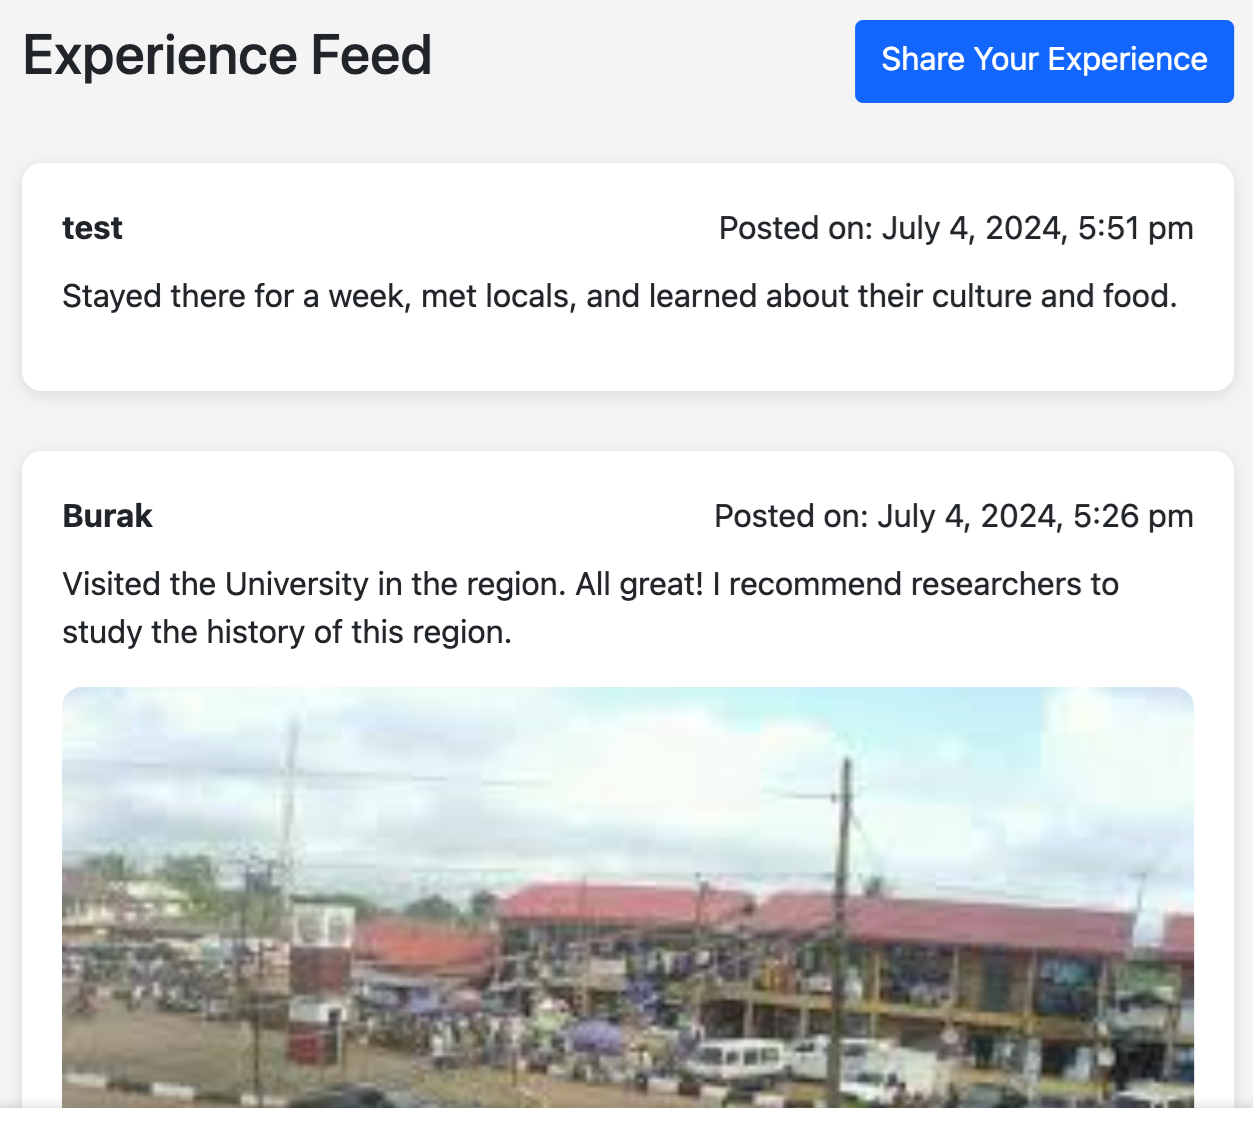
\includegraphics[width=0.5\textwidth]{experienceFeed.png}}}
		& 
		\vtop{\vskip-2ex\hbox{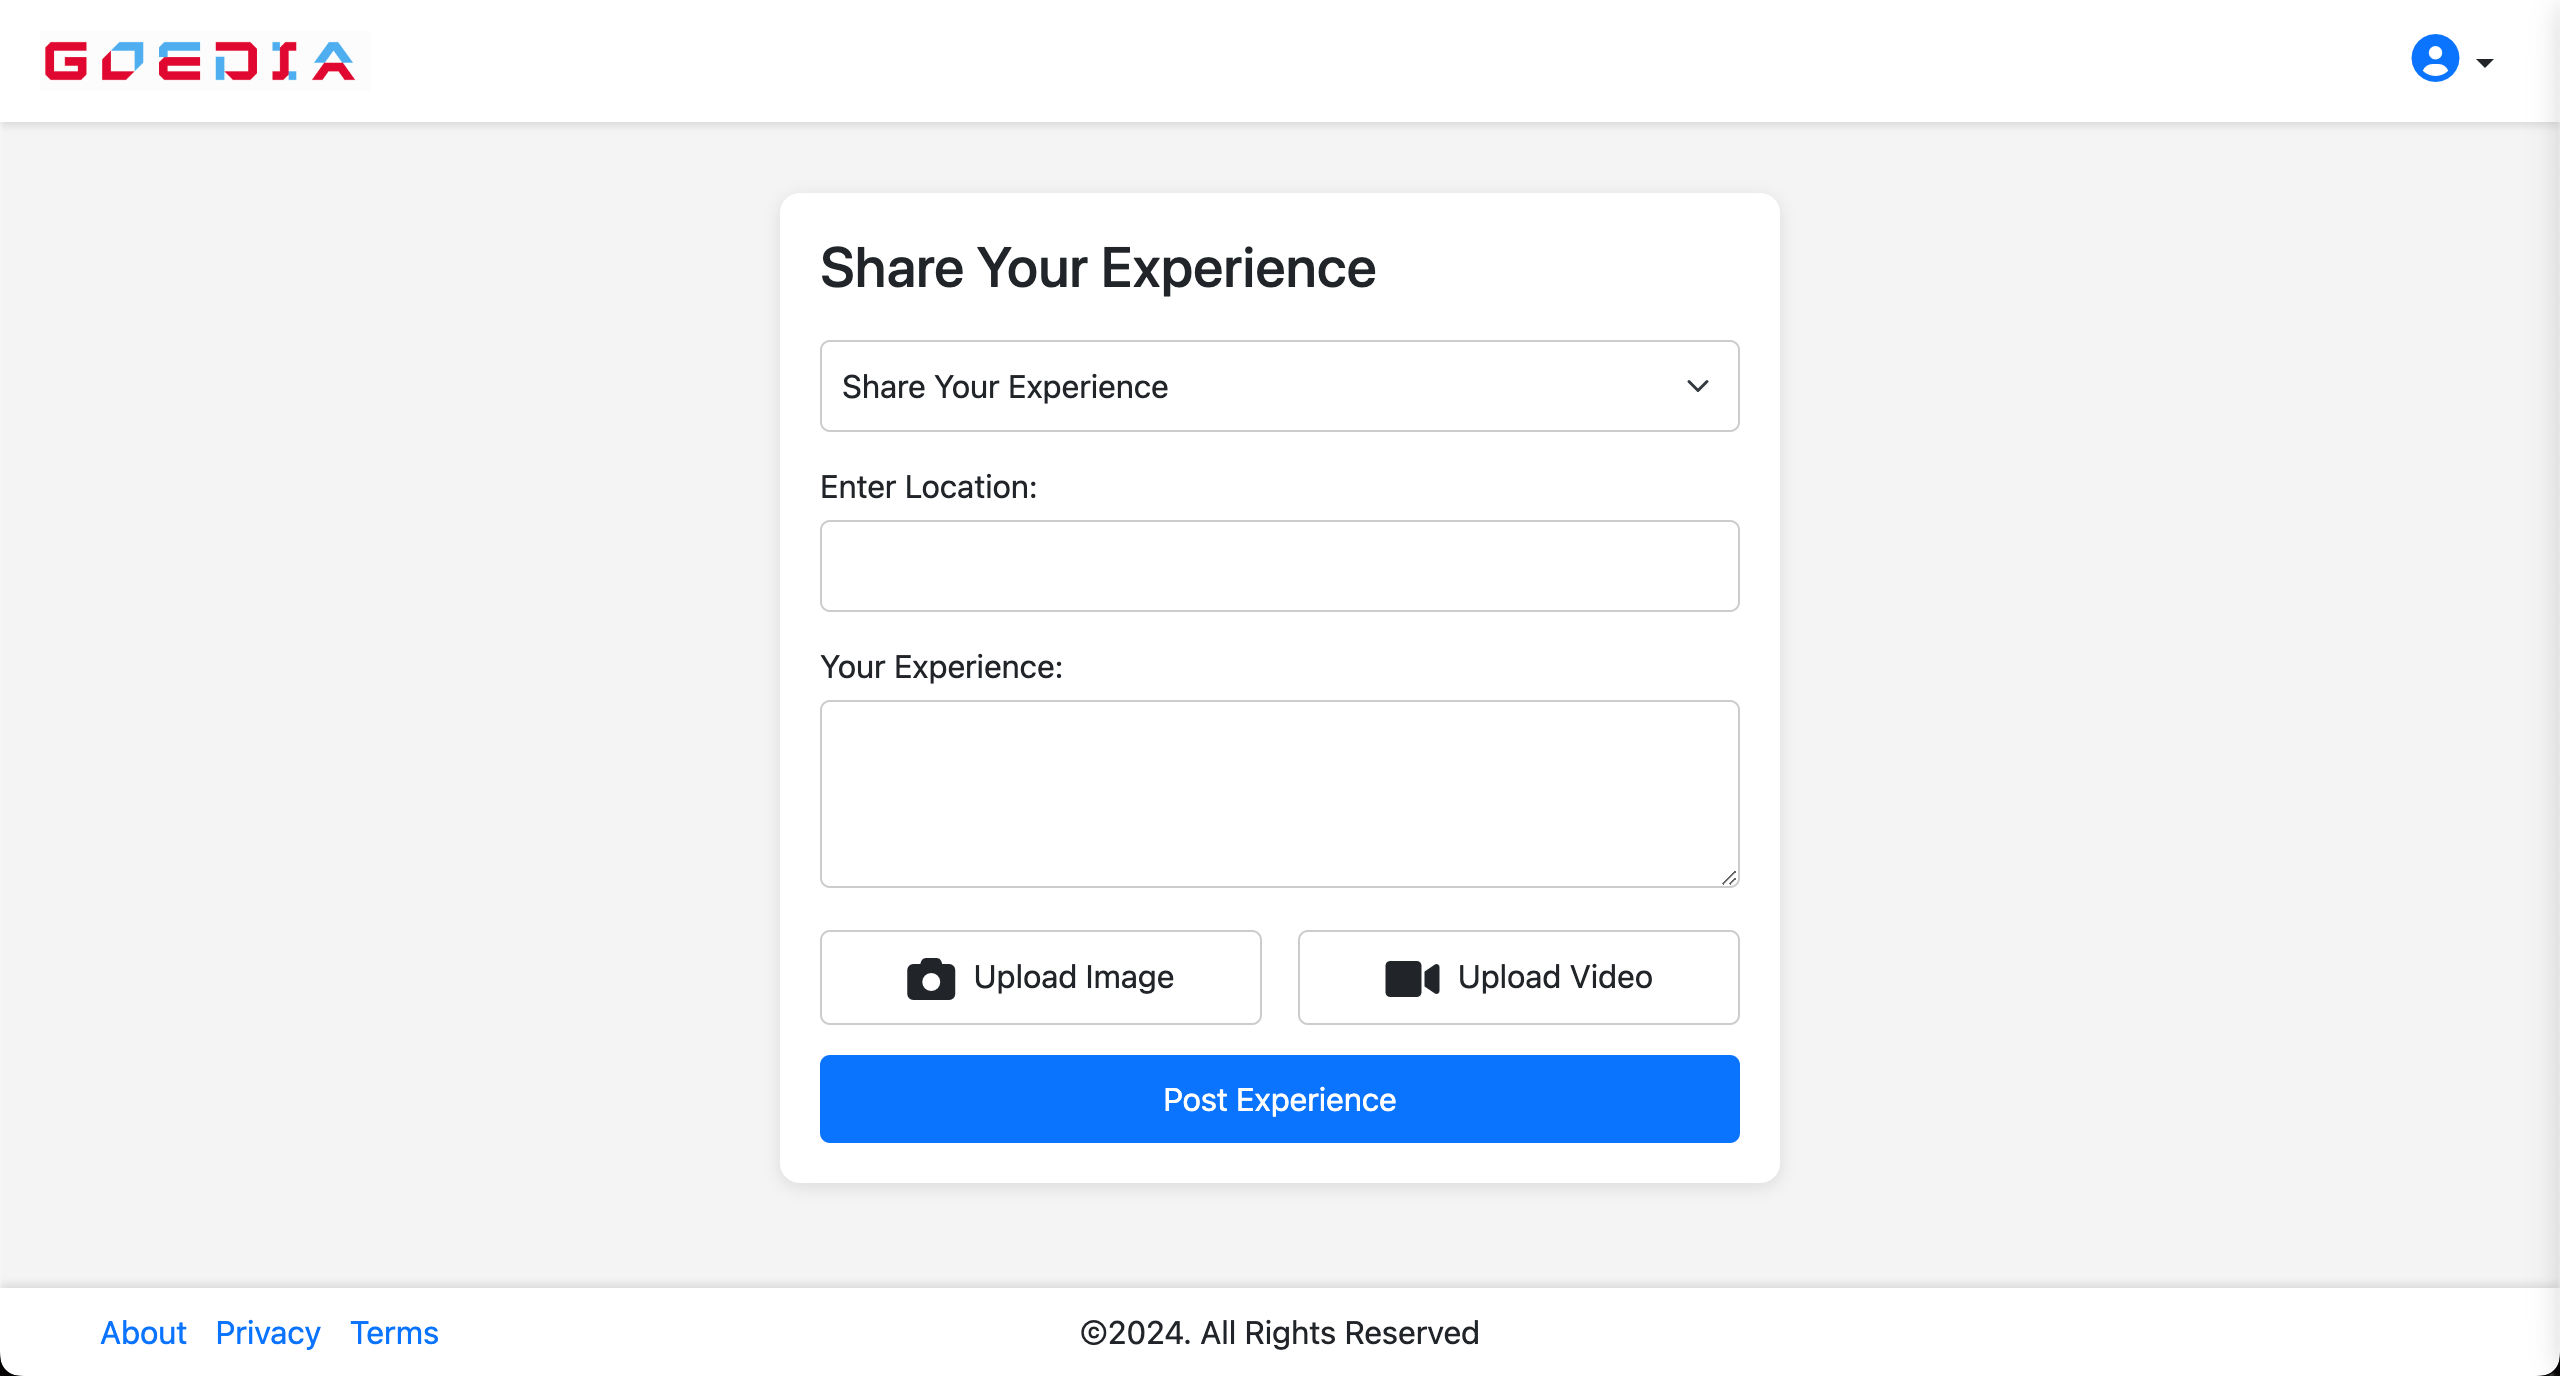
\includegraphics[width=0.4\textwidth]{shareYourexperience.png}}}
		\end{tabular}
    \caption{Experience Feed: a) feed content; b) share experience input form}
    \label{fig:experienceFeed}
\end{figure}


\section{Administrative functions of PNIS}
\subsection{Administrator Login}
Administrators have a separate login page to access additional functions for managing the application (see figure~\ref{fig:adminLogin}). This ensures secure access to administrative features.
\begin{figure}[htb]
    \centering
    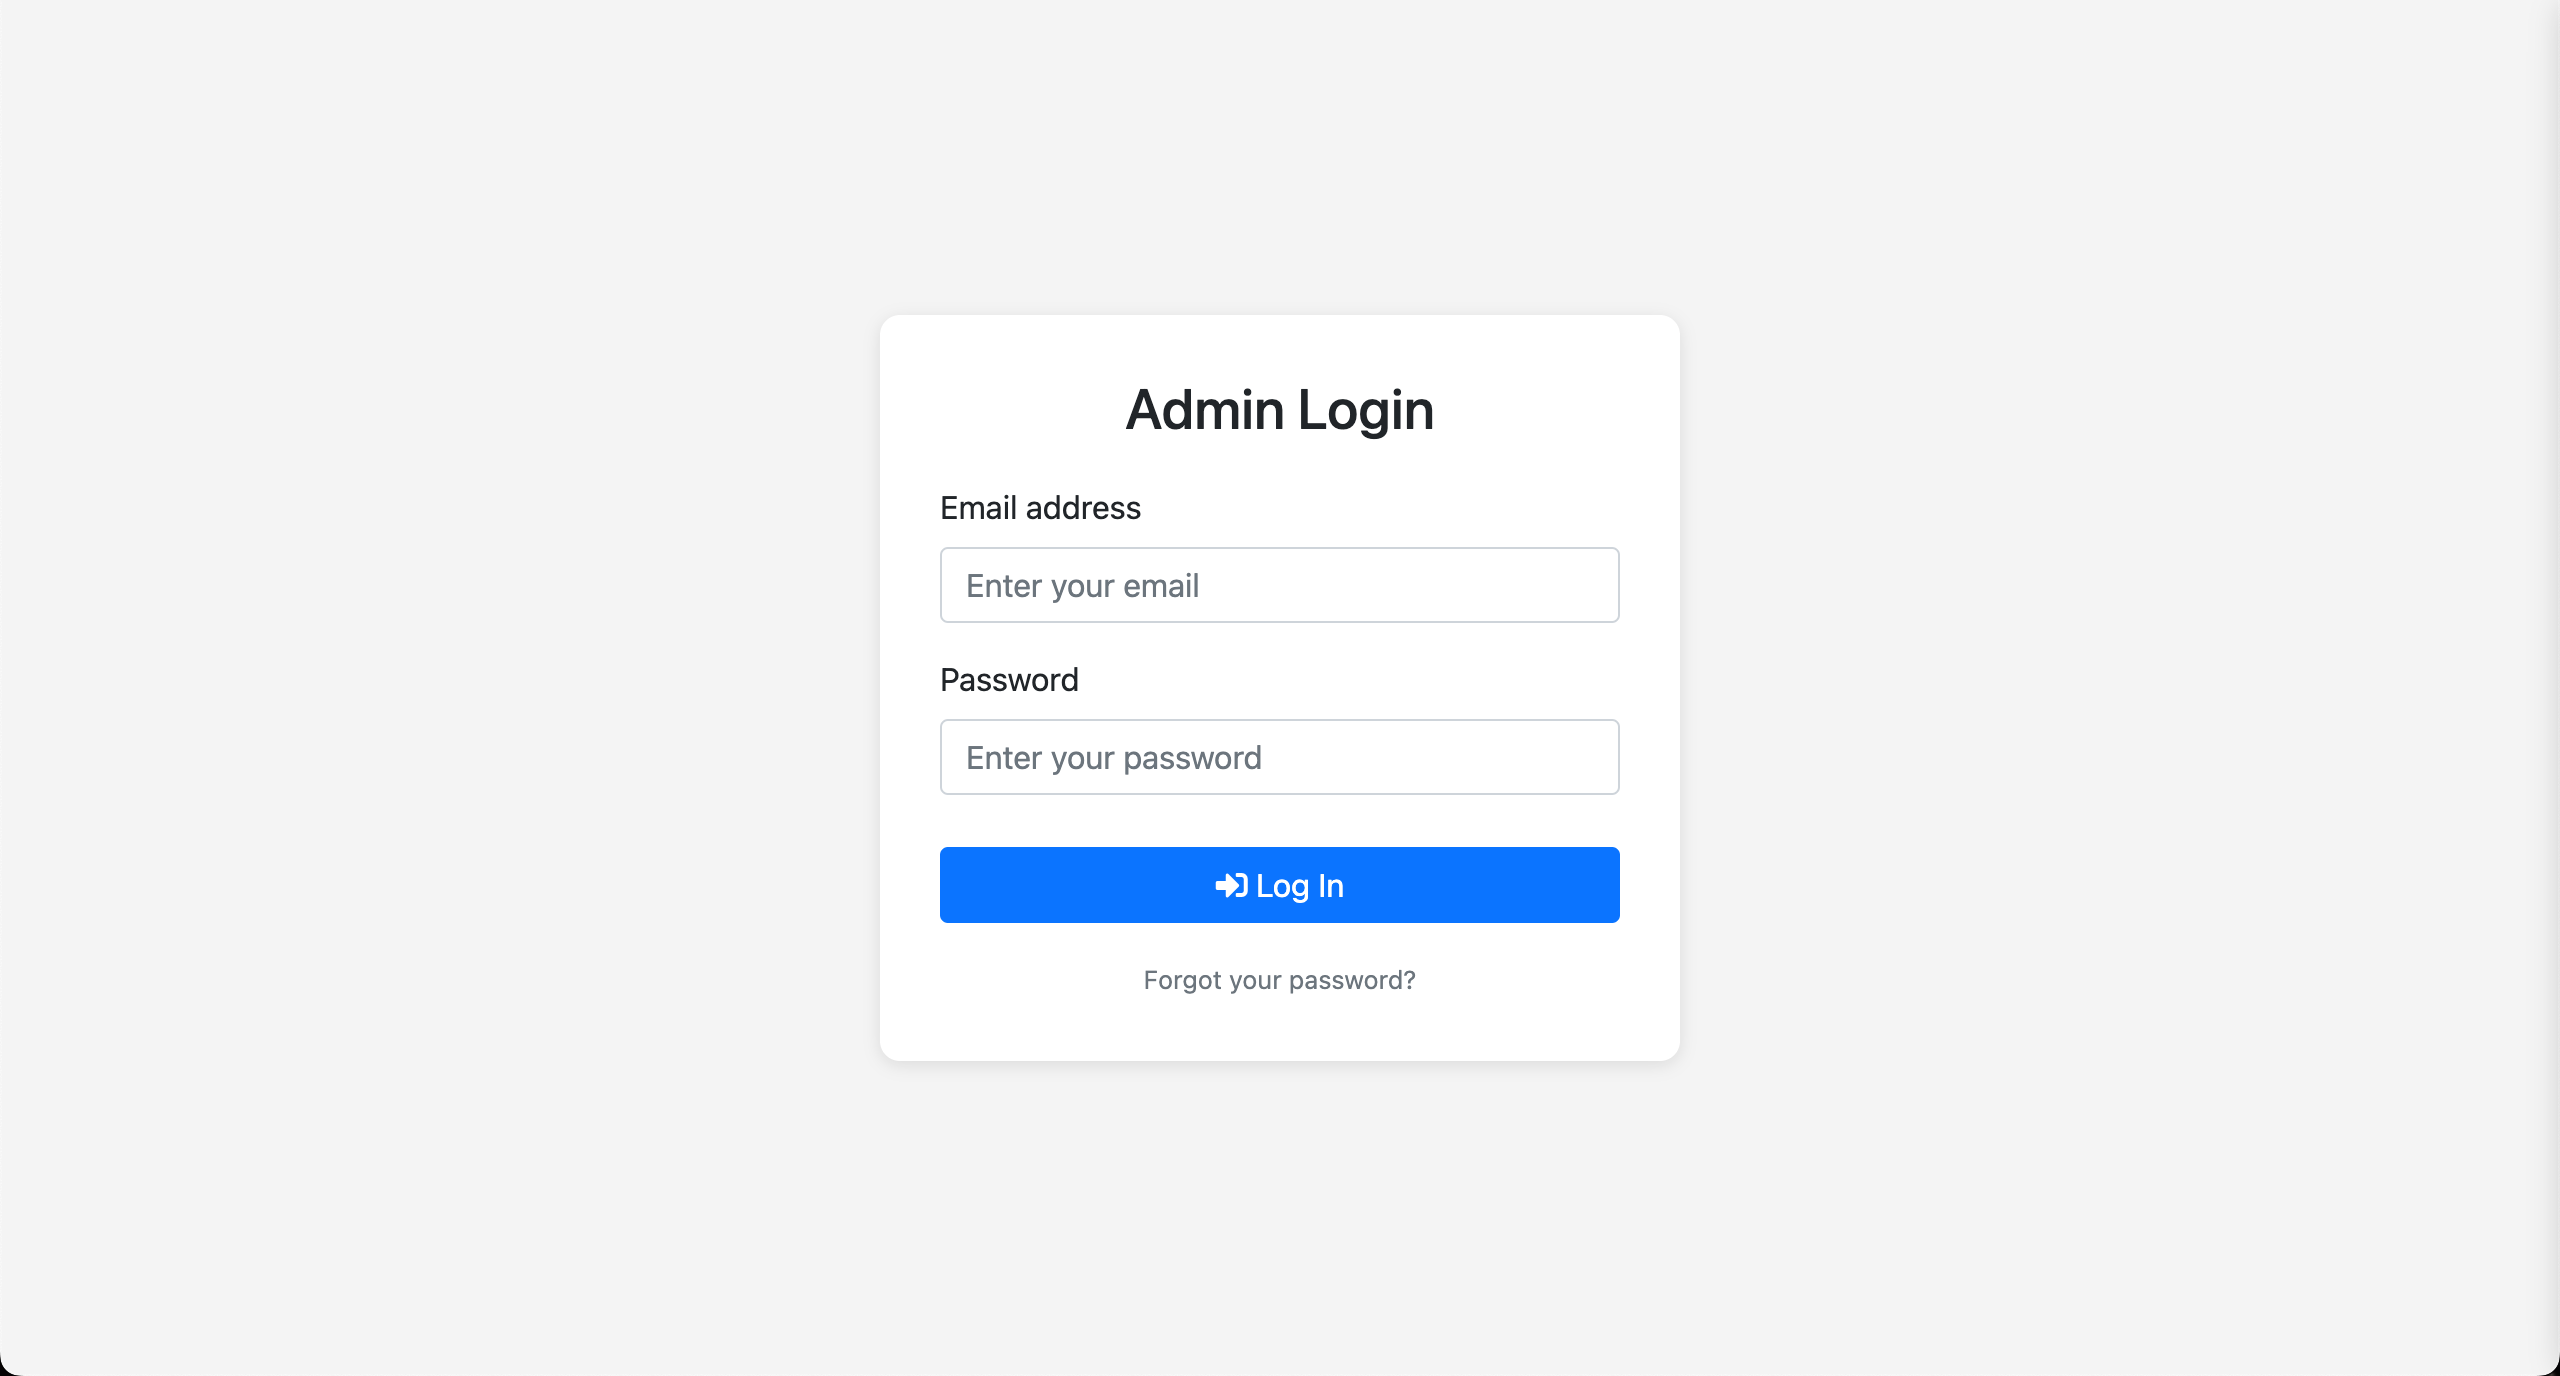
\includegraphics[width=0.4\textwidth]{adminLogin.png}
    \caption{Administrator Login}
    \label{fig:adminLogin}
\end{figure}

\subsection{Administrator Dashboard}
The admin dashboard provides an overview of various metrics and functions that administrators can manage. This includes user management, content moderation, and site analytics (see figure~\ref{fig:adminDash}).
\begin{figure}[htb]
    \centering
    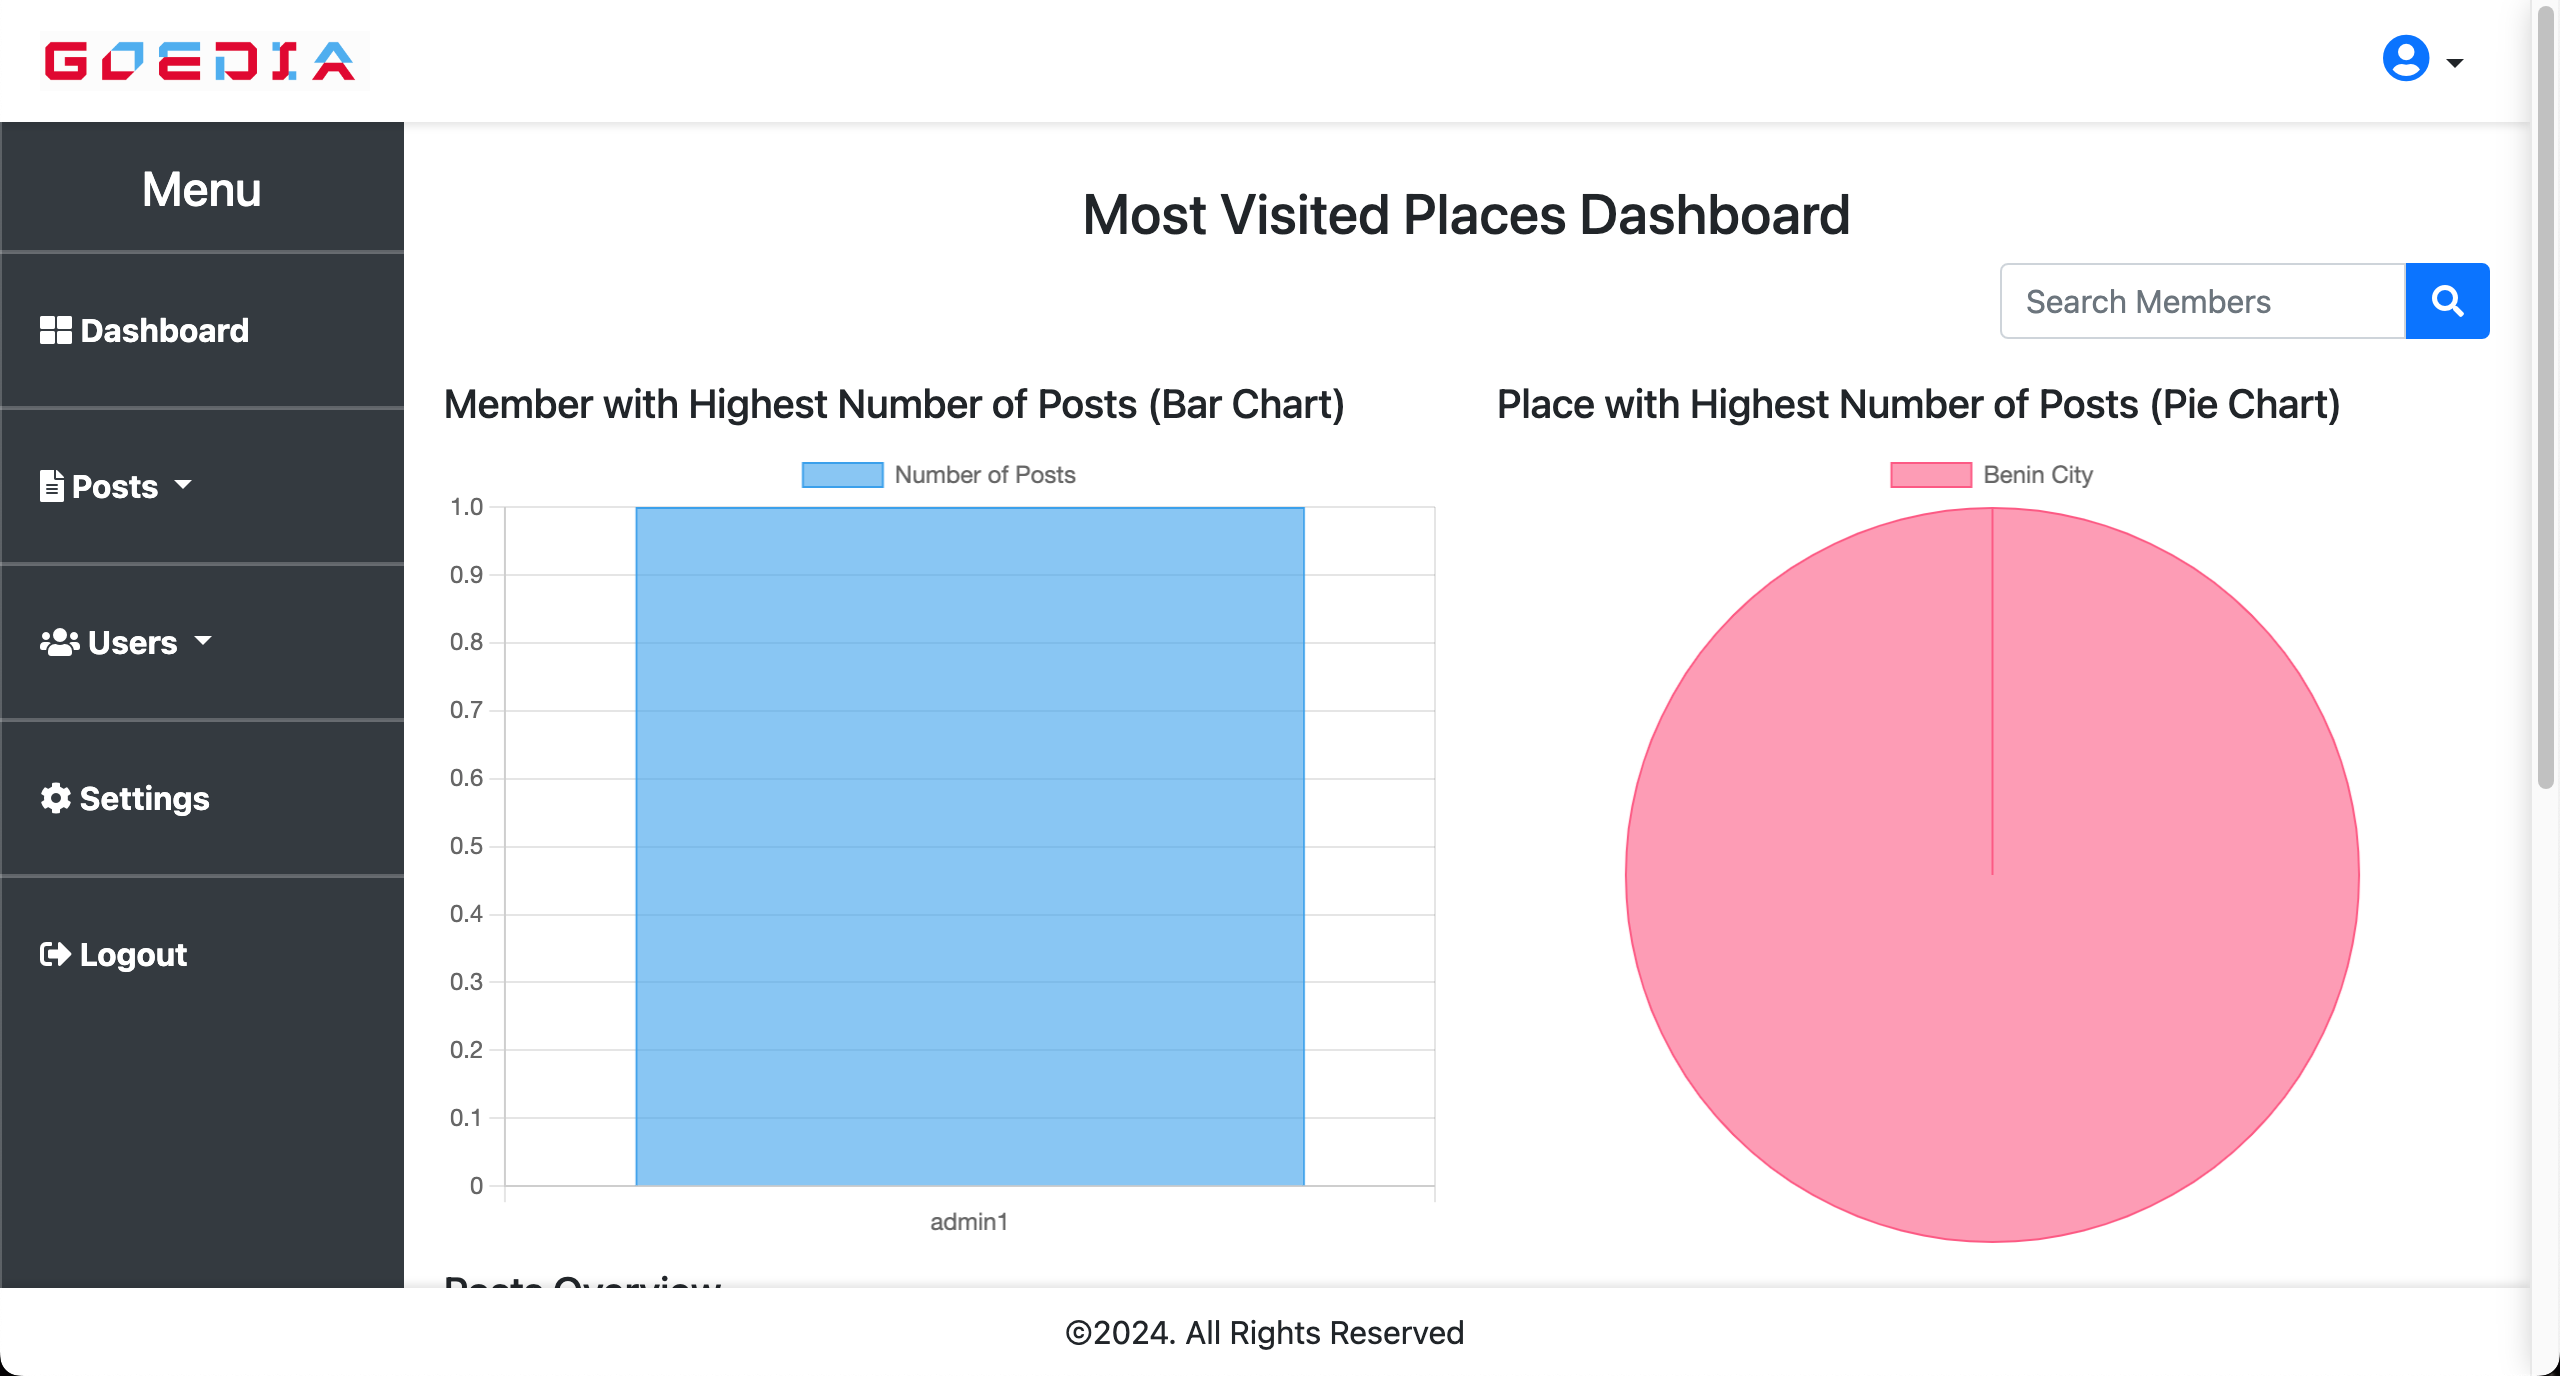
\includegraphics[width=\textwidth]{adminDash.png}
    \caption{Administrator Dashboard}
    \label{fig:adminDash}
\end{figure}

A more detailed view of the admin dashboard with additional metrics and options (see figure~\ref{fig:adminDash2}). Administrators can perform advanced tasks and get a deeper insight into the site's performance.
\begin{figure}[htb]
    \centering
    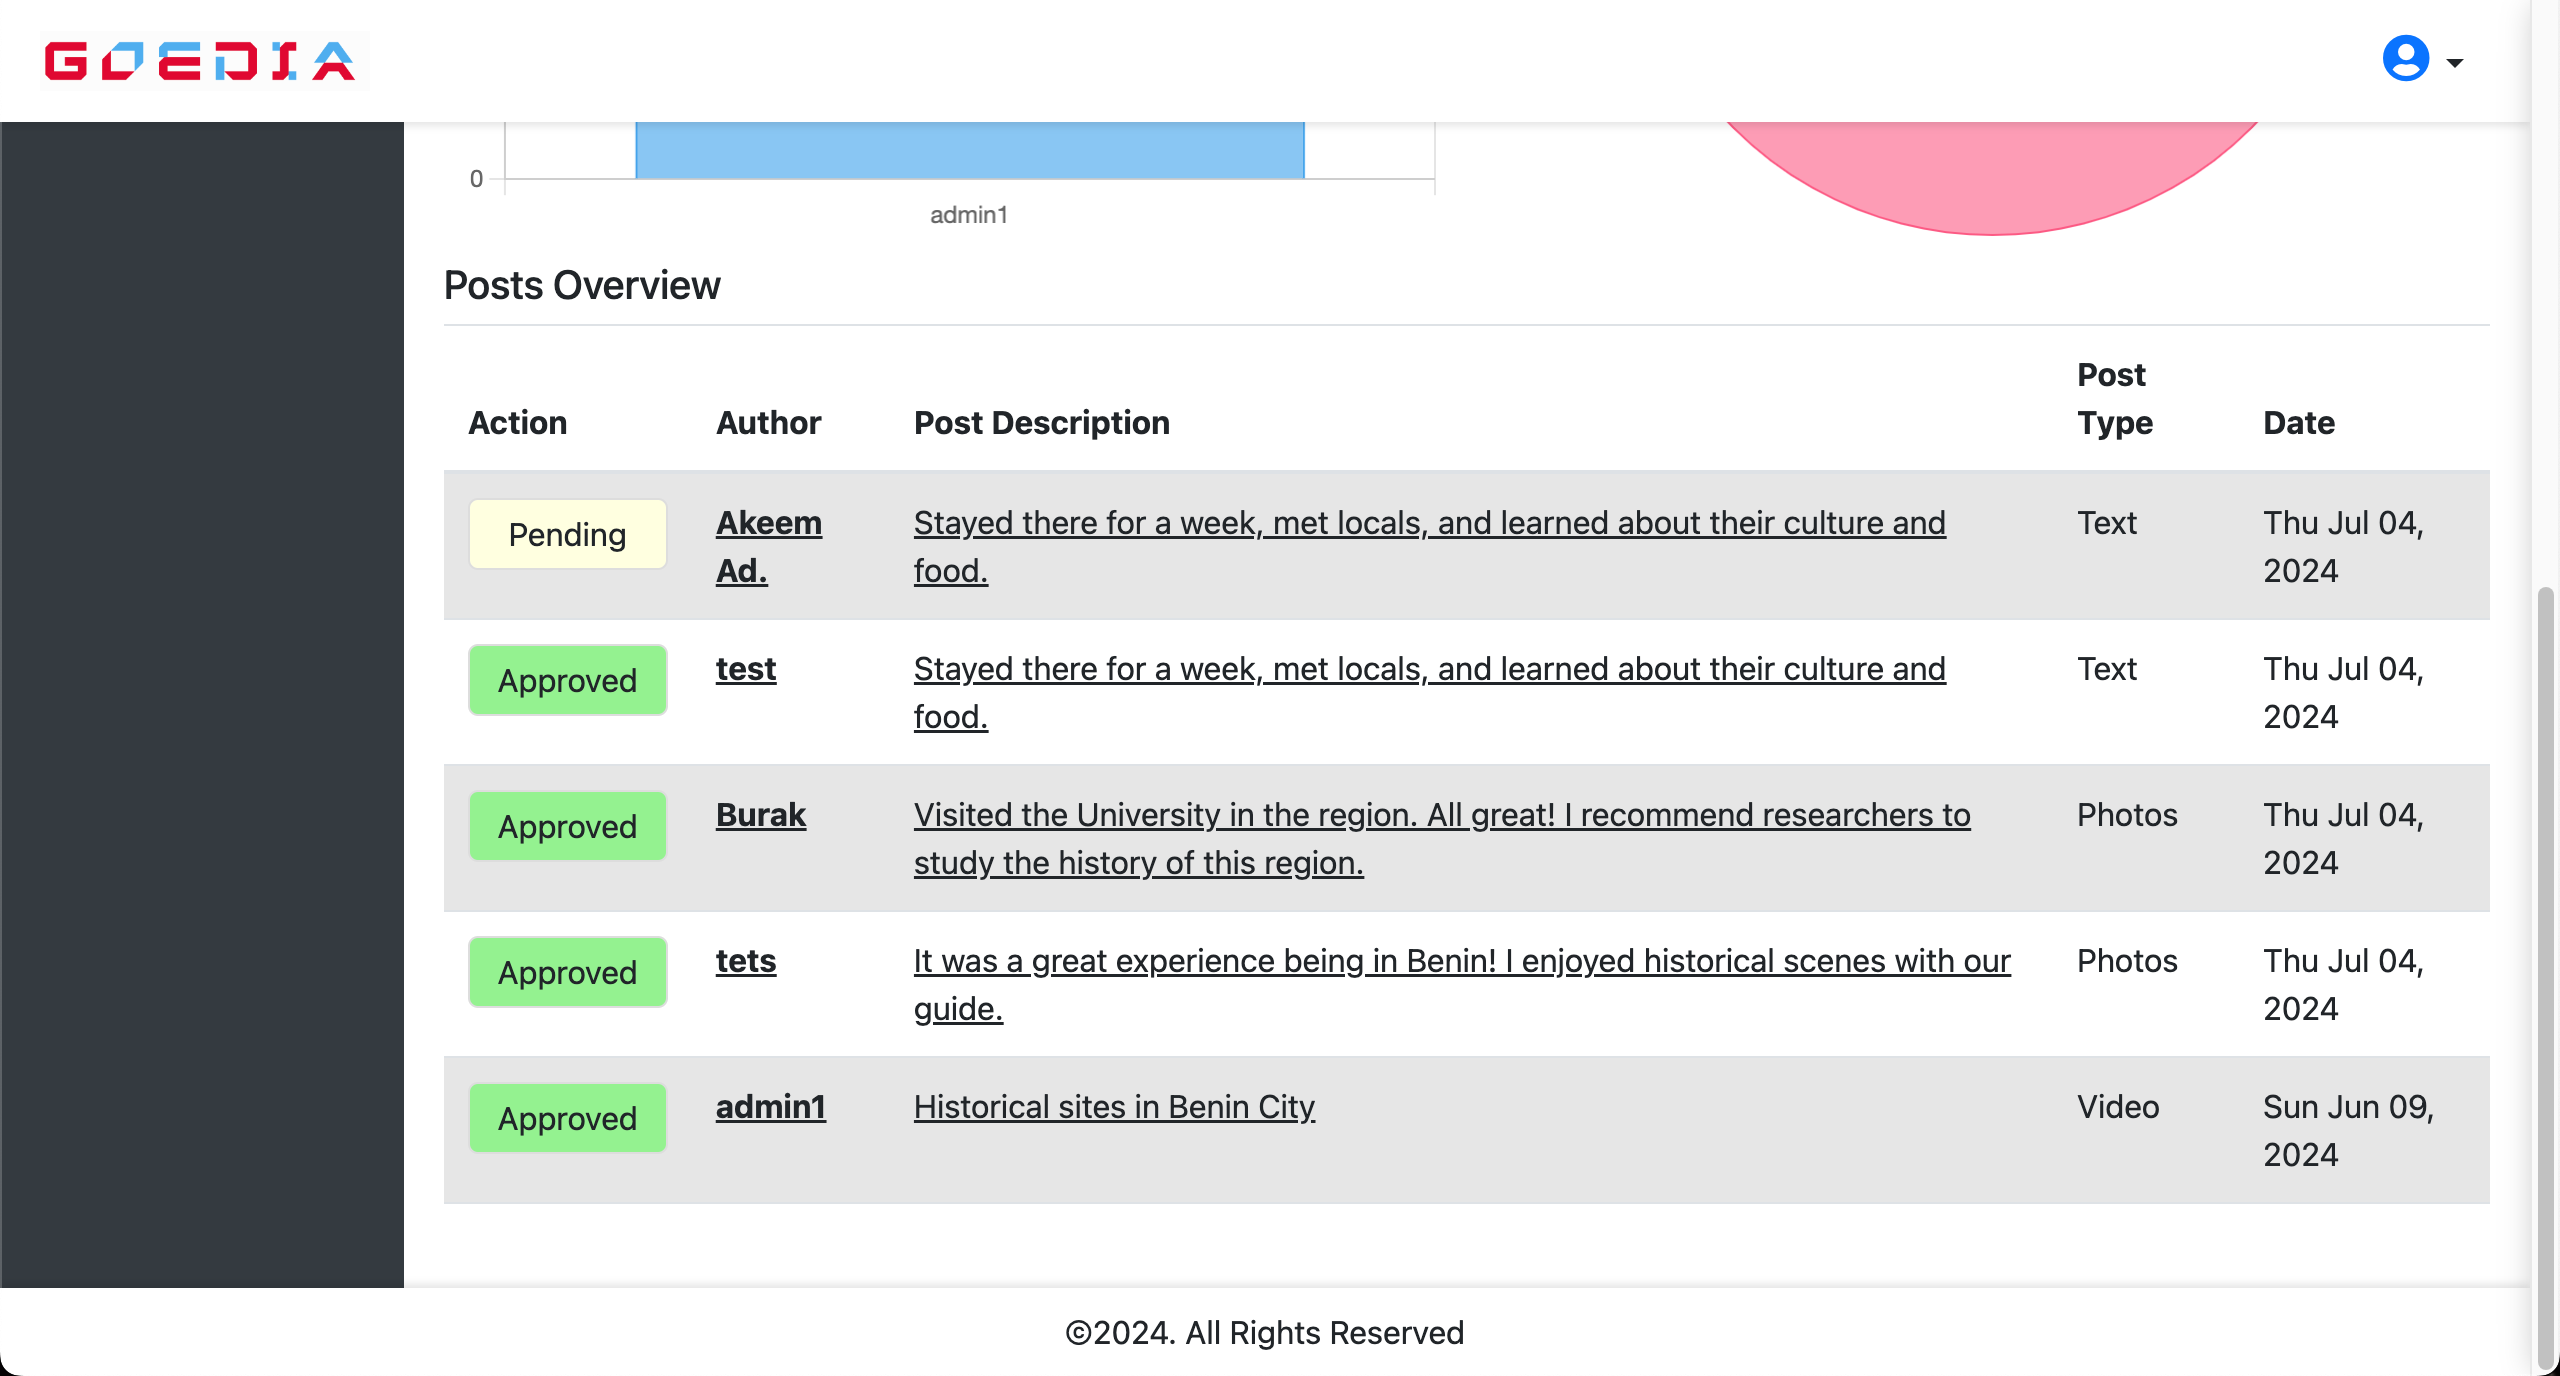
\includegraphics[width=\textwidth]{adminDash2.png}
    \caption{Administrator Dashboard - Extended View}
    \label{fig:adminDash2}
\end{figure}

\subsection{Admin Posts Management}
Administrators can manage user posts, including viewing, editing, and deleting posts if necessary (see figure~\ref{fig:adminPOSTS}). This ensures the content remains appropriate and useful for all users.
\begin{figure}[htb]
    \centering
    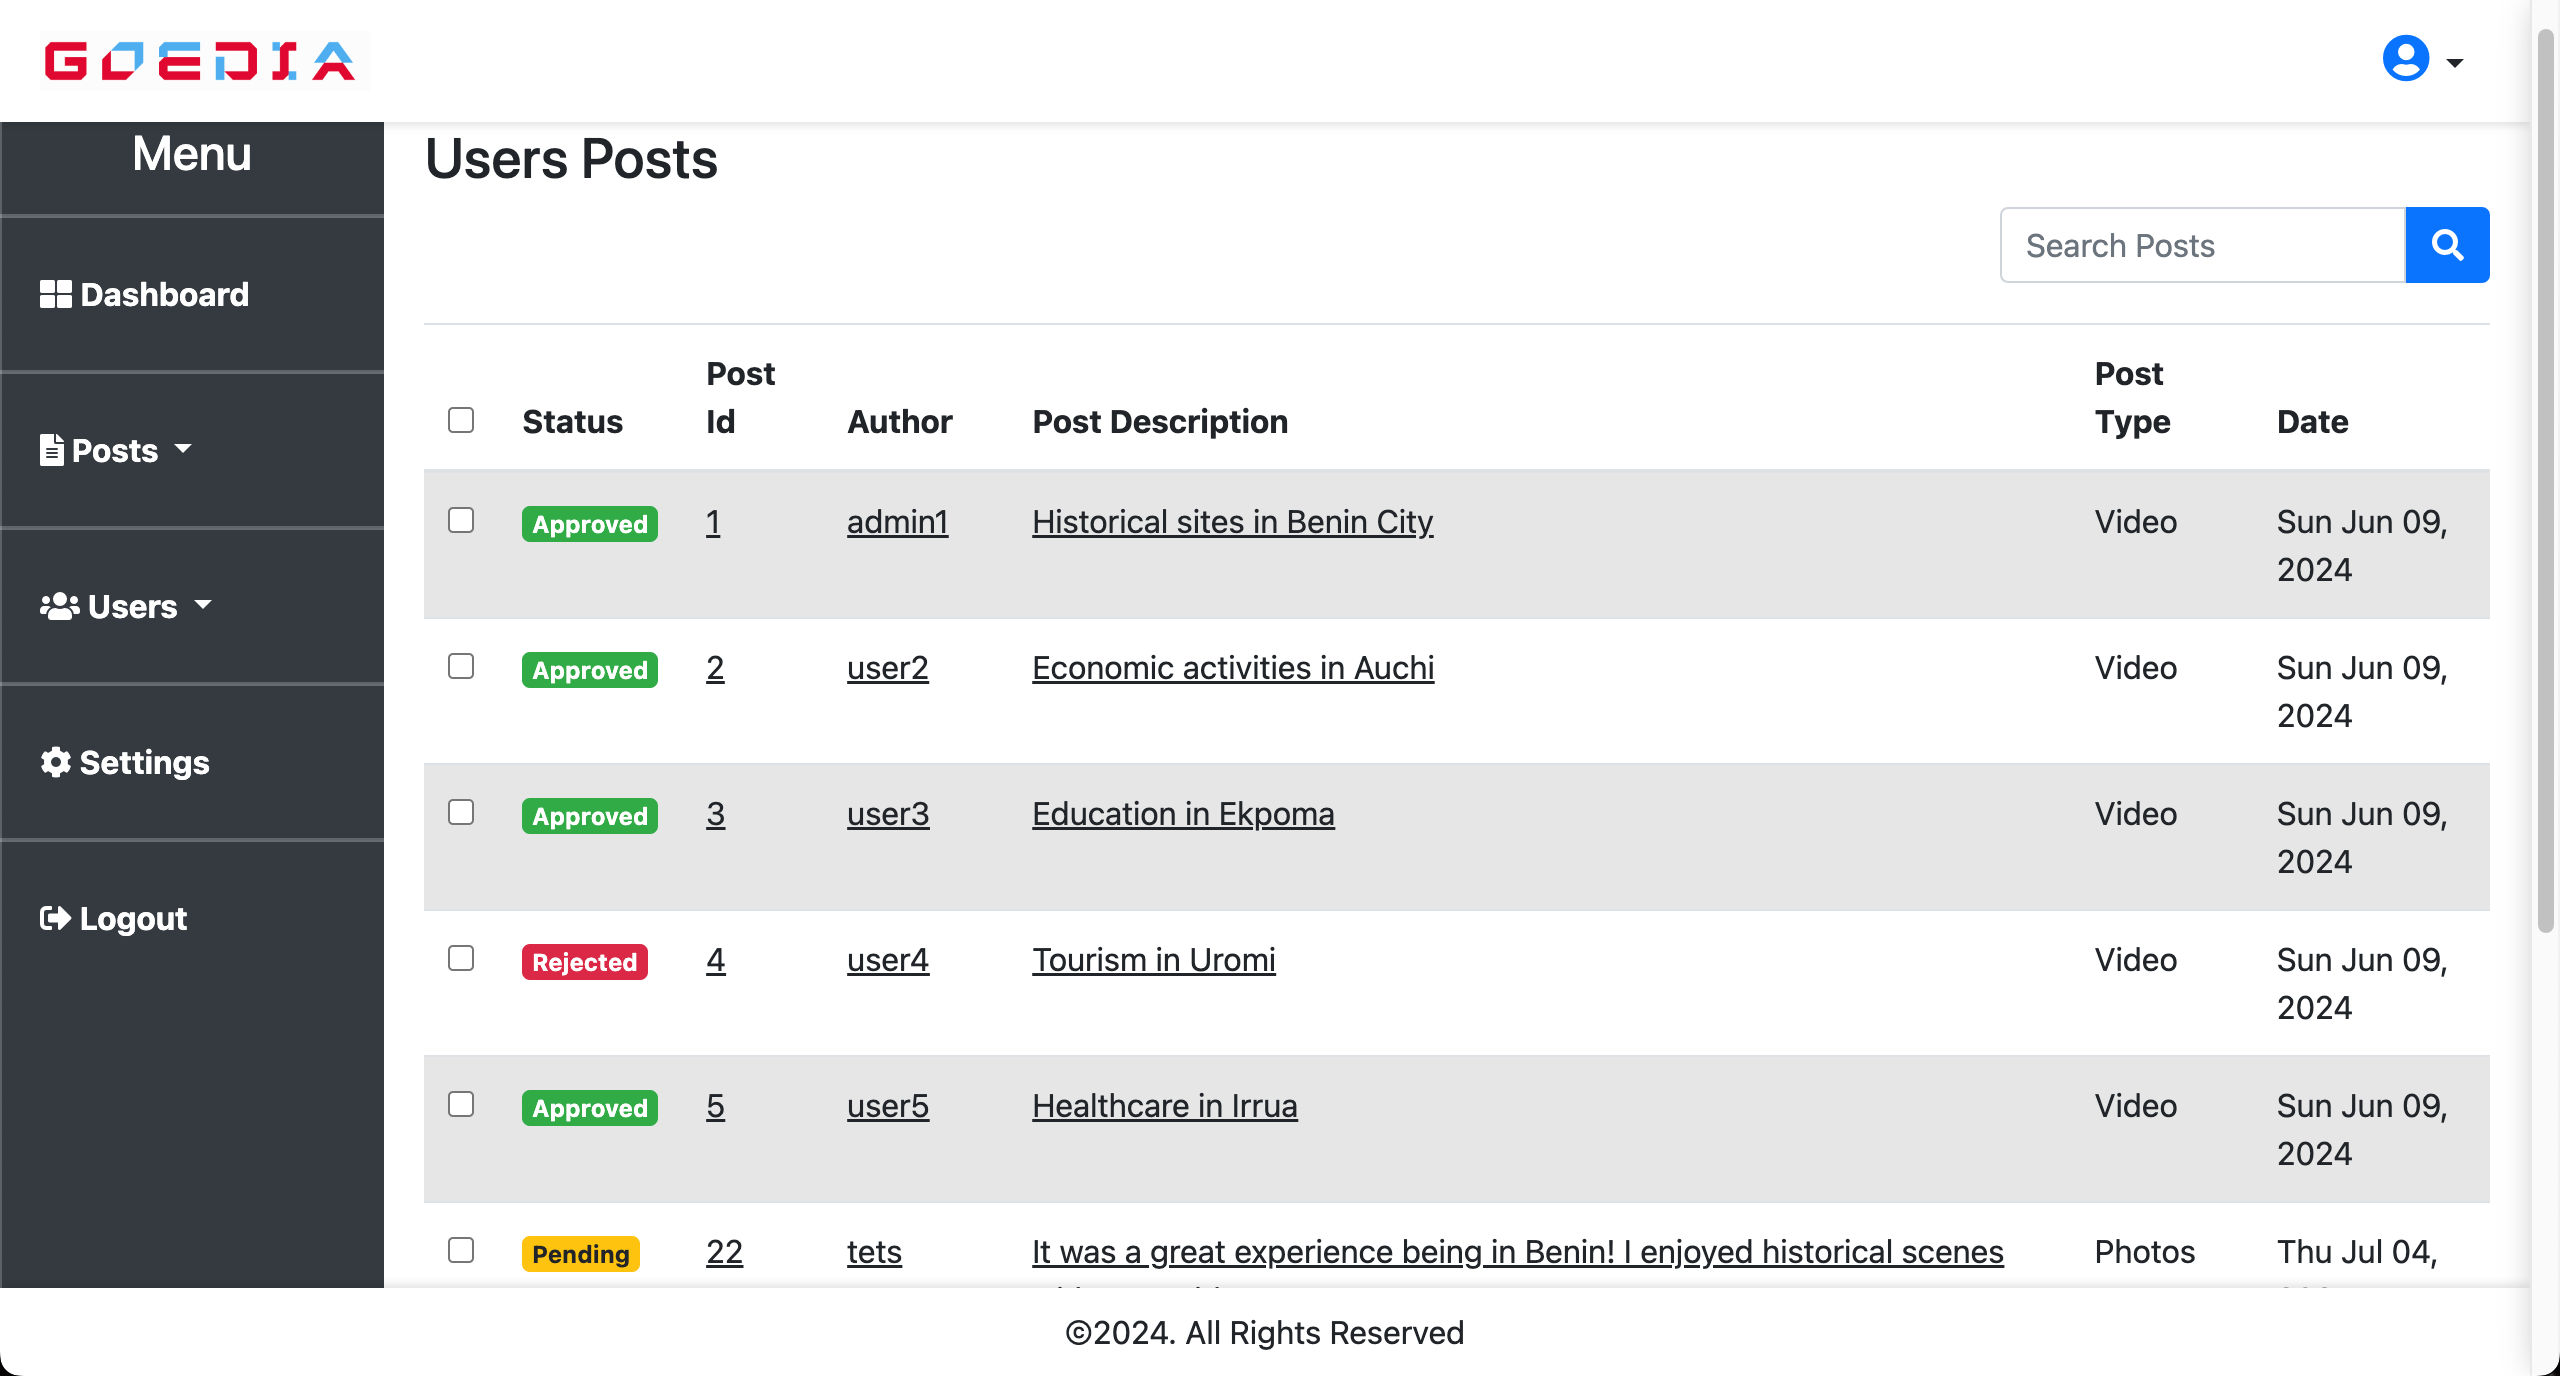
\includegraphics[width=\textwidth]{adminPOSTS.png}
    \caption{Admin Posts Management}
    \label{fig:adminPOSTS}
\end{figure}
